\documentclass{article}                     % onecolumn (standard format)
\usepackage[a4paper]{geometry}

% Line numbers
% \usepackage[left,modulo]{lineno}
% \linenumbers
% \modulolinenumbers[5]
\usepackage[ruled,vlined]{algorithm2e}
\usepackage[utf8]{inputenc}
%\usepackage{amsmath,amssymb,amsthm,mathrsfs,amsfonts,dsfont,bm}
\usepackage{amssymb}
\usepackage{amsmath}
\usepackage{dsfont}%\documentclass[a4paper,11pt]{article}
\usepackage[dvipsnames]{color,xcolor}
\usepackage{graphicx}
\usepackage{float, wrapfig}
\usepackage{empheq}
\usepackage{appendix}
\usepackage{enumerate}
\usepackage{mathtools}  
\usepackage{multirow}
\usepackage{tikz}
\usepackage{natbib}
\usepackage{setspace}
\usepackage[affil-it]{authblk} 
\usepackage{hyperref}
\usepackage{ulem}
\usetikzlibrary{shapes,backgrounds,arrows,automata,decorations,shadows,positioning, mindmap}
\newcommand*\xbar[1]{%
   \hbox{%
     \vbox{%
       \hrule height 0.5pt % The actual bar
       \kern0.5ex%         % Distance between bar and symbol
       \hbox{%
         \kern-0.1em%      % Shortening on the left side
         \ensuremath{#1}%
         \kern-0.1em%      % Shortening on the right side
       }%
     }%
   }%
} 
\newcommand{\edgeunit}{1.5}
\newcommand{\nodesize}{1em}
%\newcommand{\edgeunit}{4*\nodesize}
\newcommand{\length}{1}
\tikzstyle{covariate}=[draw, rectangle, minimum width=\nodesize, minimum height=\nodesize, inner sep=0, color=black]
\tikzstyle{covmiss}=[draw, minimum width=\nodesize, minimum height=\nodesize, inner sep=0, color=gray, text=gray]
\tikzstyle{observed}=[draw, circle, minimum width=\nodesize, inner sep=0, color=black]
\tikzstyle{basic}=[draw, circle, minimum width=0.4*\nodesize, inner sep=0, color=black, fill=black]
\tikzstyle{clique}=[draw, rectangle, minimum width=2*\nodesize, minimum height=2*\nodesize, inner sep=0, color=black]
\tikzstyle{edge}=[-, line width=1pt, color=black]
\tikzstyle{edgemiss}=[-, line width=1pt, dashed, color=gray]
\tikzstyle{variable}=[scale=0.9,rectangle,draw=white,transform shape,fill=white,font=\Large]
    

%%%%%%%%%%%%%%%%%%%%%%%%%%%%%%%%%%%%%%%%%%%%%
%% Environment
\renewcommand{\appendixname}{Annex}
\newtheorem{theorem}{Theorem}
\newtheorem{lemma}{Lemma}
\newtheorem{remark}{Remark}
\renewcommand{\abstractname}{Summary} 
\definecolor{red1}{RGB}{228,26,28}
\definecolor{red2}{RGB}{251,180,174}
\definecolor{blue1}{RGB}{55,126,184}
\definecolor{blue2}{RGB}{179,205,227}
\definecolor{aqua2}{RGB}{0,161,108}
\definecolor{aqua1}{RGB}{151,217,195}

 
\newcommand{\RM}[2]{\textcolor{aqua1}{\sout{#1}}\textcolor{aqua2}{#2}} % Raph
\newcommand{\SR}[2]{\textcolor{gray}{#1}\textcolor{blue}{#2}} % SR

\newcommand\independent{\protect\mathpalette{\protect\independenT}{\perp}}
\newcommand{\STAB}[1]{\begin{tabular}{@{}c@{}}#1\end{tabular}}

% Functions
\def\independenT#1#2{\mathrel{\rlap{$#1#2$}\mkern2mu{#1#2}}}
\DeclareMathOperator*{\argmax}{arg\,max}
\DeclareMathOperator*{\argmin}{arg\,min}
\DeclareMathOperator*{\Esp}{\mathbb{E}}
\DeclareMathOperator*{\Var}{\mathbb{V}}
\DeclareMathOperator*{\Cov}{\mathbb{C}\text{ov}}
\DeclareMathOperator*{\prob}{\mathds{P}}
\DeclareMathOperator*{\probt}{\widetilde{\mathds{P}}}

% Notations pairs
\newcommand\jk{{jk}}

% Notations cal
\newcommand\Ccal{\mathcal{C}}
\newcommand\Ncal{\mathcal{N}}
\newcommand\Pcal{\mathcal{P}}
\newcommand\Tcal{\mathcal{T}}
\newcommand\mt{\widetilde{m}}
\newcommand\St{\widetilde{S}}
\newcommand\mbt{\widetilde{\bf m}}
\newcommand\Sbt{\widetilde{\bf S}}

% Notations bf
\newcommand\gammab{{\boldsymbol{\gamma}}}
\newcommand\betab{{\boldsymbol{\beta}}}
\newcommand\thetab{{\boldsymbol{\theta}}}
\newcommand\Sigmab{{\boldsymbol{\Sigma}}}
\newcommand\cst{\text{cst}}
\newcommand\Ob{{\bf O}}
\newcommand\Hb{{\bf H}}
\newcommand\Mb{{\bf M}}
\newcommand\Qb{{\bf Q}}
\newcommand\Wb{{\bf W}}
\newcommand\Xb{{\bf X}}
\newcommand\xb{{\bf x}}
\newcommand\Yb{{\bf Y}}
\newcommand\Zb{{\bf Z}}
\newcommand\zb{{\bf z}}



% Notations tilde
\newcommand\Pt{\widetilde{P}}
\newcommand\pt{\widetilde{p}}
\newcommand\et{\widetilde{\mathds{E}}}
\newcommand\e{{\mathds{E}}}
% TikZ
\newcommand{\nodesize}{1em}
\newcommand{\edgeunit}{4*\nodesize}
\tikzstyle{covariate}=[draw, rectangle, minimum width=\nodesize, minimum height=\nodesize, inner sep=0, color=black]
\tikzstyle{covmiss}=[draw, minimum width=\nodesize, minimum height=\nodesize, inner sep=0, color=gray, text=gray]
\tikzstyle{observed}=[draw, circle, minimum width=\nodesize, inner sep=0, color=black]
\tikzstyle{edge}=[-, line width=1pt, color=black]
\tikzstyle{edgemiss}=[-, line width=1pt, dashed, color=gray]

\newcommand{\argmin}{\arg\!\min}
\newcommand{\argmax}{\arg\!\max}
\newcommand{\tr}{\text{tr}}
\newcommand*\widefbox[1]{\fbox{\hspace{3em}#1\hspace{3em}}}
\newcommand*\lesswidefbox[1]{\fbox{\hspace{2em}#1\hspace{2em}}}
\newcommand{\entr}{\mathcal{H}}
\newcommand{\betat}{{\widetilde{\beta}}}
\newcommand{\Bt}{{\widetilde{B}}}
\newcommand{\Pt}{{\widetilde{P}}}
\newcommand\Ibb{\mathbb{I}}
\newcommand{\betabf}{{\boldsymbol{\beta}}}
\newcommand{\thetabf}{{\boldsymbol{\theta}}}
\newcommand{\sigmabf}{{\boldsymbol{\sigma}}}
%\newcommand{\mubf}{\boldsymbol{\mu}}
\newcommand{\Omegabf}{{\boldsymbol{\Omega}}}
\newcommand{\Sigmabf}{{\boldsymbol{\Sigma}}}
\newcommand{\Gammabf}{{\boldsymbol{\Gamma}}}
\newcommand{\zerobf}{{\boldsymbol{0}}}
\newcommand{\Xbf}{{\boldsymbol{X}}}
\newcommand{\xbf}{{\boldsymbol{x}}}
\newcommand{\Ybf}{{\boldsymbol{Y}}}
\newcommand{\Zbf}{{\boldsymbol{Z}}}
\newcommand{\Wbf}{{\boldsymbol{W}}}
\newcommand{\Ubf}{{\boldsymbol{U}}}
\newcommand{\Mbf}{{\boldsymbol{M}}}
\newcommand{\Qbf}{{\boldsymbol{Q}}}
\newcommand{\Rbf}{{\boldsymbol{R}}}
\newcommand{\Sbf}{{\boldsymbol{S}}}
\newcommand{\mbf}{{\boldsymbol{m}}}
\newcommand\Ccal{{\mathcal{C}}}
\newcommand\Hcal{{\mathcal{H}}}
\newcommand\Jcal{{\mathcal{J}}}
\newcommand\Ncal{{\mathcal{N}}}
\newcommand\Pcal{{\mathcal{P}}}
\newcommand\Tcal{{\mathcal{T}} }
\newcommand{\Cor}{{\mathds{C}\text{or}}}
\newcommand{\Esp}{{\mathds{E}}}
\newcommand{\Var}{{\mathds{V}}}
\newcommand{\bound}{{\mathcal{J}}}
% \newcommand{\corTemp}{{\Cor_{\text{temp}}}}
\newcommand{\corHTemp}{{\rho(H, \text{temp})}}
\newcommand{\corKTemp}{{\rho(k, \text{temp})}}

\newcommand{\betabft}{{\widetilde{\betabf}}}
\newcommand{\Mbft}{{\widetilde{\Mbf}}}
\newcommand{\Sbft}{{\widetilde{\Sbf}}}


\newtheorem{theorem}{Theorem}
\newtheorem{lemma}{Lemma}

\definecolor{azure}{rgb}{0.0, 0.5, 1.0}
\definecolor{blue2}{rgb}{0.16, 0.32, 0.75} 
\newcommand{\RM}[2]{\textcolor{gray}{#1}\textcolor{blue2}{#2}}
\newcommand{\CA}[2]{\textcolor{gray}{\sout{#1}}\textcolor{Peach}{#2}}
\newcommand{\SR}[2]{\textcolor{black}{\sout{#1}}\textcolor{blue}{#2}}

%JRSSC authors guidlines:
%- not more than 24 journal pages
%- computations in appendices
%- matrices in italic and vectors in bold
%- short summary (100 words), with 5 to 6 keywords
%- no pb with arXiv
%%%%%%%%%%%%%%%%%%%%%%%%%%%%%%%%%%%%%%%%%%%%%

\title{\textbf{Accounting for missing actors in interaction network inference from abundance data}}

\author{Raphaëlle Momal$^1$%
  \thanks{Electronic address: \texttt{raphaelle.momal@agroparistech.fr}; Corresponding author}, \hspace{0.3cm} Stéphane Robin$^2$, \hspace{0.3cm} Christophe Ambroise$^3$}
\affil{1: UMR MIA-Paris, AgroParisTech, INRAE, Université Paris-Saclay, Paris, France.\\
2: CESCO, Muséum National d'Histoire Naturelle, CNRS, Sorbonne Université, Paris, France.\\
3: Université Paris-Saclay, CNRS, Univ. Évry, Laboratoire de Mathématiques et Modélisation d’Évry 91037, \'Evry, France.}

\date{\today}

\begin{document}

\maketitle
\begin{abstract}
%\SR{Network inference is used in many areas such as genomics or ecology to infer the structure of conditional independence between covariates, based on the measures of gene expression or species abundance for example. In many experiments, it is likely that not all covariates involved in the network were actually observed. Then observed samples are drawn from a distribution where some unobserved covariates were marginalized.
%
%We introduce a generic statistical model for network inference from abundance data with missing actor. The model includes fixed effects to take account of environmental covariates  and sampling efforts, as well as correlated random effects to encode species interactions. The correlation structure is that of a Gaussian graphical model marginalized on one ore more covariates, corresponding to the missing actors. The inferred network is obtained by averaging on all spanning trees, in a computationally efficient way.}{}
% \SR{
% % 25 mots 
% Network inference aims at  unraveling  the dependency structure  relating  jointly observed  variables. Graphical models provides a flexible framework for identifying variables that are {\sl directly related}.
% %  10 mots 
% Unobserved variables  ({\sl missing actors}) may induce an apparent 
% direct dependency.
% % 28 mots
% In the context of abundance data, we introduce a model based on the Poisson log-normal distribution, and  a tree-based approach,  to recover the dependency structure  including missing actors.
% % 27 mots
% The  performances of the proposed variational EM estimation algorithm 
% are assessed via synthetic data. Using  ecological datasets, we  demonstrate the  ability of our approach to recover environmental drivers.
% % 8 mots
% The corresponding R package is available
% from \url{https://github.com/Rmomal/VEMtree}. 
% }{
Network inference aims at unraveling the dependency structure relating jointly observed variables. Graphical models provide a general framework to distinguish between marginal and conditional dependency.
Unobserved variables ({\sl missing actors}) may induce apparent conditional dependencies.
In the context of count data, we introduce a mixture of Poisson log-normal distributions with tree-shaped graphical models, to recover the dependency structure, including missing actors. 
We design a variational EM algorithm and assess its performance on synthetic data. We demonstrate the ability of our approach to recover environmental drivers on two ecological datasets.
The corresponding R package is available from \url{github.com/Rmomal/nestor}.\\
%}
%%%%% \CA{}{98 mots}

%\RM{}{D'après les guidelines: 100 mots max pour le résumé.}\\
%\RM{}{La package est disponible à \url{https://github.com/Rmomal/VEMtree}.}
\paragraph{Keywords:}graphical models, network inference, missing actor, abundance data, Variational EM algorithm, matrix tree theorem, Poisson log-Normal model
\end{abstract}

% \SR{}{
% \begin{itemize}
% \item Parler de l'identifiabilité
% % \item revoir l'argumentaire arbre / Chow-Liu
% \end{itemize}}
 \newpage
% intro
%Les réseaux :
%- [ ] C’est quoi
%- [ ] À quoi ça sert (les enjeux, appliqué)
%- [ ] Quelles sont les questions qui se posent (que dit la recherche)
%
%- [ ] Lauritzen pour les nuls
%
%L’inférence de réseaux :
%- [ ] Quelle méthode pour quel réseau
%- [ ] Auxquelles on se compare, pourquoi elles sont comme ça comment elles marchent et ce qui manque

  \section*{Biological context}
 \subsection*{Networks}
 A network is an intuitive object which anyone can easily relate to. It is first of all a graphical tool representing the links between different entities. This helps understand how a system organizes and have a direct image of it. It is also an analysis tool which can unravel sensible information about the system, its structure and the different roles in its organization. Networks are versatile tools that are  used in many domains (e.g. sociology, linguistics, computer sciences, neurosciences, climatology, psychology, etc.) and can take various forms to adapt to each problem.  They can be directed or undirected. Some link entities with multiple kinds of edges (multidimensional), or have different layers (multiplex), others link groups of disconnected objects (multipartite). In biology, the most typical networks simply represent the species (nodes) and their relationships (edges).

Various types of species interactions are studied with networks. For example, their is a rich literature of networks for plant-pollinator and host-parasite relationships in ecology. These species interactions are clearly defined and directly observed in the field. Contacts of pollination or parasitism are counted and networks constructed from these interaction abundances.
\begin{figure}
\centering
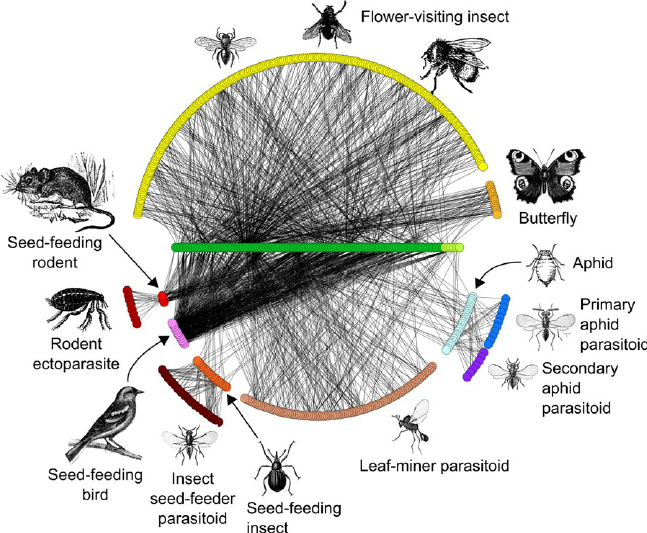
\includegraphics[width=0.7\linewidth]{figs/pocock.png}
\caption{Species interaction networks at Norwood Farm, Somerset, UK \citep{PED12,BRM13}.}
\label{pocock}
\end{figure}
 However many mechanisms cannot be observed and may not be well defined. One way to discover them may then be to resort to a more mathematical definition of species interactions. Working with the latter allows the study of community assembly mechanisms with the inference of networks representing guilds of species in community ecology. This type of network is extensively used in genomics for protein-protein interaction network, or gene regulatory networks, or in microbiology to study the output of a metabarcoding experiment assessing the composition of a microbiome. 
 
 \begin{figure}
\centering
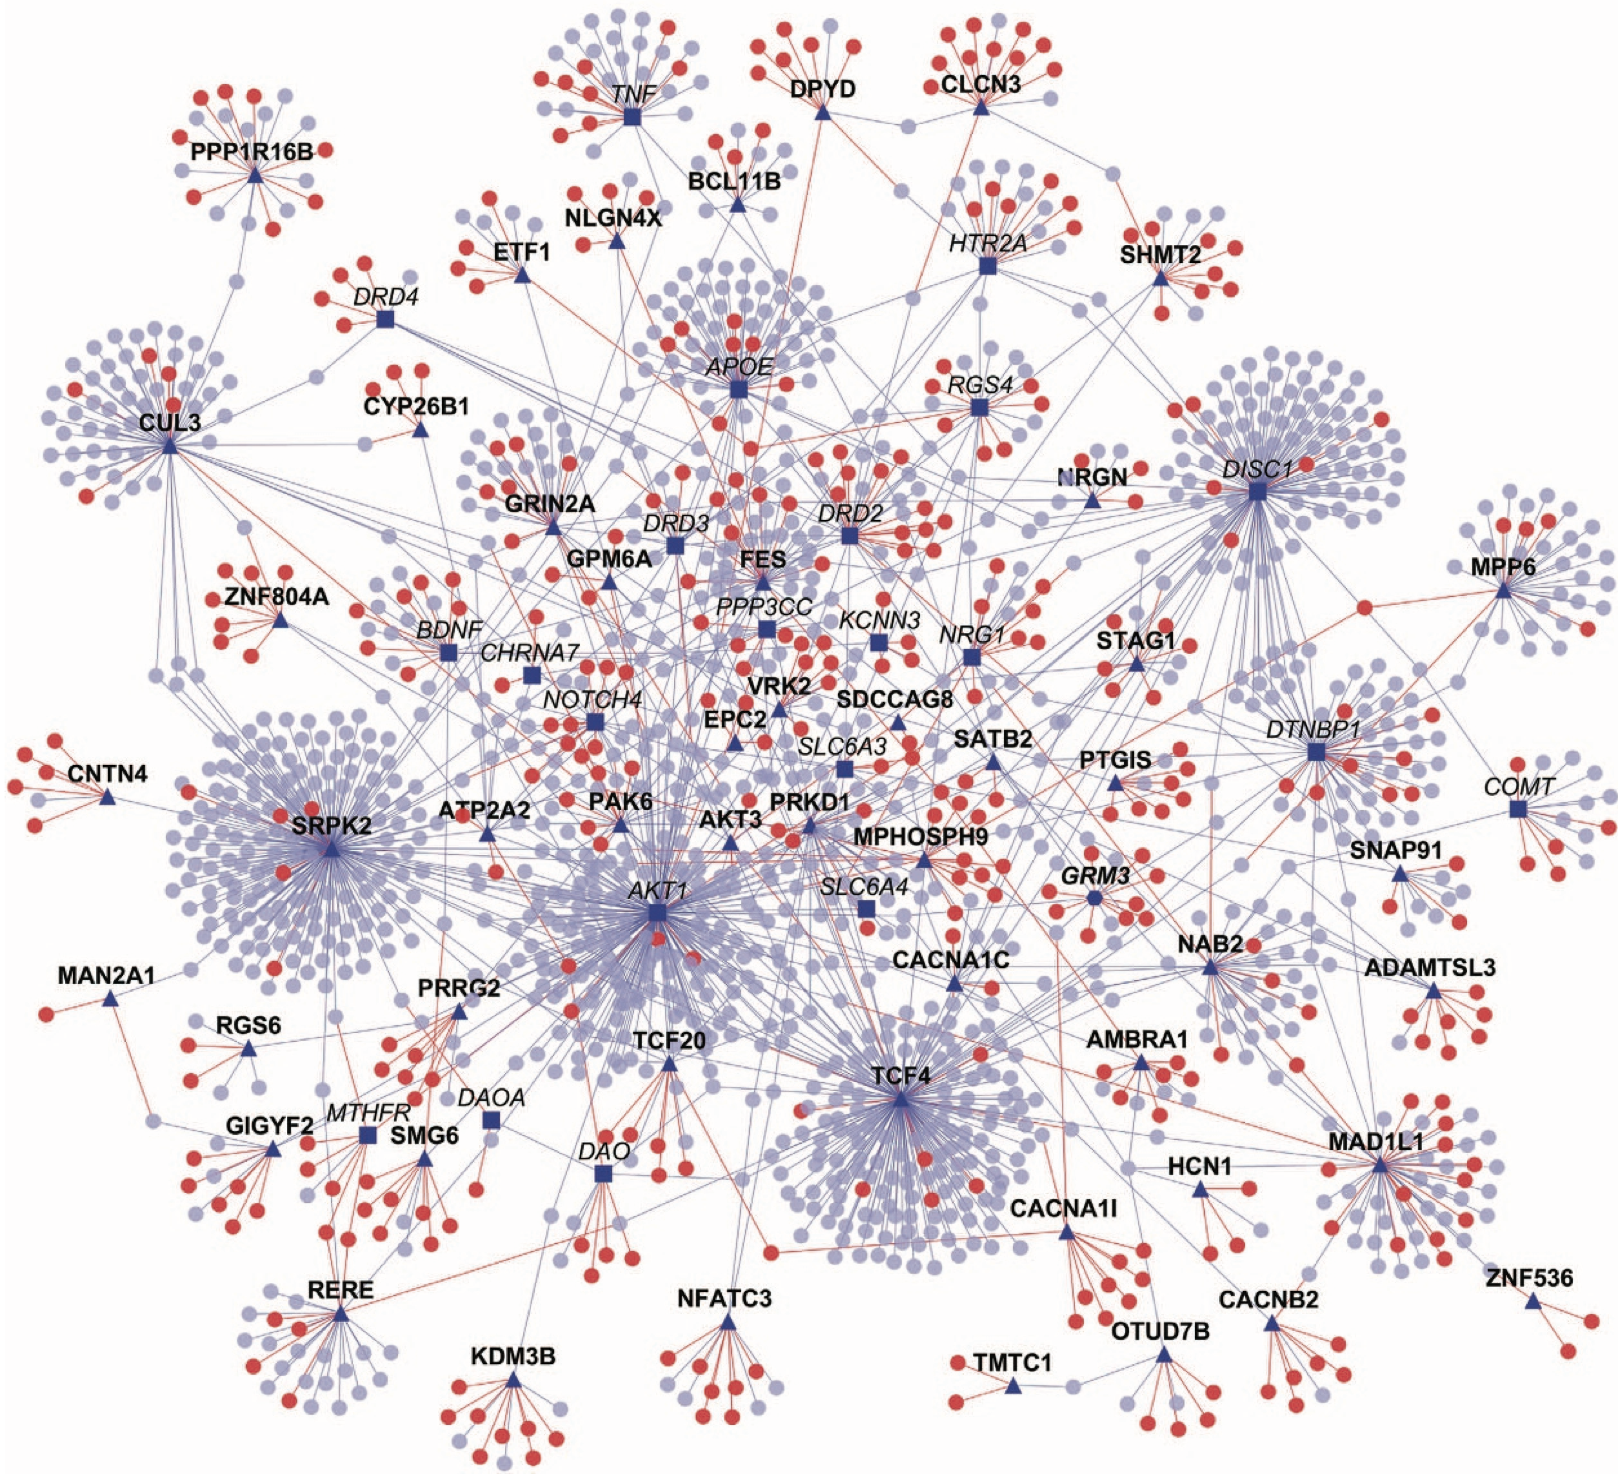
\includegraphics[width=0.7\linewidth]{figs/PPInetwork.png}
\caption{Protein-protein interactions between genes involved in schizophrenia \citep{GTH16}.}
\label{PPI}
\end{figure}

  \subsection*{Statistical interactions}
The correlations between the species measures first come to mind as a statistical characterization of an interaction. These are easily obtained, yet their corresponding networks are hard to interpret. Indeed, two covariates correlating with a same third one will appear correlated, even if they have no direct effect on each other\footnote{e.g. the number of covid 19 cases detected correlates with both the real number of cases and the number of tests done on the population, which induces a spurious correlation between the two latter where obviously there is no direct effect of one on the other.}. This phenomena of spurious correlations complicates both the analysis and the interpretation by inducing a very high number of edges  which cannot be categorized as direct or indirect associations between the species. 
 
 Conditional dependencies are then very useful measures of interaction. They describe dependencies between each pair of species conditional on all others. That is, all other species measures kept fixed, their measures should still be correlated. A link between two species can then be interpreted as a direct association. This yields a network of species conditional dependence (link) and independence (absence of link), which is interpretable and falls within the well-studied mathematical framework of graphical models.
 
 \subsection*{Measures on species}
 Networks of statistical interactions are obtained from datasets of repeated measures on a set of species, which can be of various types. Measures can be continuous, as for example the output of gene expression profiling experiments using DNA microarrays, which  are  fluorescences measures from targeted genes. Using a Gaussian approximation, these measures of genes expressions can be used to derive genes regulatory networks.  Measures can also be binary, as in co-occurrence data in ecology, which record the joint presences and absences of a set of species in several sites. \citet{CAM16}.
%développer les données de co-occurence

Abundance data  are joint counts of species in a series of sites (also known as assemblages data in ecology). Recent technologies made this type of data increasingly available. Assemblages data were rare in ecology as they implied intensive sampling efforts, which is now greatly facilitated by camera traps and sensors. In metagenomics, high-throughput sequencing technologies for metabarcoding experiments made it possible  to get joint counts of pseudo-species (operational taxonomic units (OTUs)) abundances.  Both domains work with the same type of output: a dataset of joint (pseudo-)species abundances from different sites or samples.\\
%développer les metabarcoding et OTU


Once the data has been collected, it is very likely that not all species or covariates were observed: there exists missing actors and data is incomplete. In the network, the existence of a missing actor translates into appearance of edges between all the species it should connect with, creating dense cliques of species which are not actually conditionally dependent on one another. A second objective of this work is to take missing actors into account during network inference in order to get more accurate interpretations.

\section*{Network inference}
% ce qui existe et motivation du sujet
\section*{Objectives}
 \subsection*{Graphical models and Trees}
The dedicated framework for the representation of conditional dependency structures are graphical models. Gaussian Graphical Models (GGM) in particular provide with appealing algebraic properties for network inference, which are detailed in \citet{Lau96}. Exploring the set of possible graphs is a non-ending task, and we chose to reduce the searching space to that of spanning trees. This is the sparsest connected structure, and enjoys specific algebraic properties allowing to sum on all possible spanning trees at the cost of a determinant calculus. Our network inference methodology relies on spanning trees and \citet{Lau96} maximum likelihood estimators for multivariate Gaussian graphical models.

%caser le missing actor qq part
 \subsection*{Modeling abundance data}
 As this ideal framework of GGM is not directly applicable to abundance data, there exist two possible ways to proceed: either apply a Gaussian transformation to the data, or rely on Gaussian latent vectors in the framework of Joint Species Distribution Models (JSDM). Our methodology resorts to the latter, and more specifically to the Poisson log-normal distribution to model the counts. This distribution allows easy handling of both covariates and offsets, as well as take overdispersion into account thanks to its Gaussian random parameters. 
 
 
 \subsection*{Estimation procedure} %or algorithm
The central model we adopt involves a Gaussian layer of parameters which is a mixture on all spanning trees. Each component of the mixture is a Gaussian distribution which dependency structure is a spanning tree. This represents two hidden layers of parameters, which we first estimates with an Estimation-Maximization (EM) algorithm. Then to infer missing actors of the network, we resort to a variational (VEM) approach.

\section*{Outline} 
  \subsection*{Chapter 1}
The first chapter details the mathematical tools and technical results for the statistical modeling and the network inference used in Chapters 2 and 3.

   \subsection*{Chapter 2}
   This chapter details a method to infer undirected networks representing conditional statistical dependencies between the species from their joint abundance measures.  The proposed methodology, implemented in the R package \texttt{EMtree},  is compared to state of the art approaches and applied to two empirical datasets from ecology and metagenomics. This chapter has been published as an article in the journal \textit{Methods in Ecology and Evolution} \citep{MRA20}.
   
    \subsection*{Chapter 3}
This chapter details a variational approach to the inference of a missing actor in the network. The reconstruction of missing actor(s) is implemented in the R package \texttt{nestor} and illustrated on two  empirical datasets from ecology. This chapter has been submitted for publication in the \textit{Journal of the Royal Statistical Society: series C (applied statistics)}.
 
  \subsection*{Chapter 4}
This final chapter introduces some natural perspectives of this work. After concluding on the specifics of the developed methodology, natural extension are presented, including network comparison. The inclusion of spatialized data is discussed, as well as the possibility of network inference directly from the observed counts.
 \section*{Notations}
 
 \begin{description}
 \item[Operations:]  \begin{itemize}
     \item[]
 \item[] $|\cdot|$ : matrix determinant
 \item[] $\odot$ : Hadamard product
 \end{itemize}
 \item[Variables:] \begin{itemize}
     \item[]
 \item[] $\Ybf$ :  matrix  of observed counts
 \item[] $\Zbf$ : matrix of latent Gaussian parameters 
 \item[] $\Ubf$ : matrix of latent normalized Gaussian parameters 
 \item[] $\Xbf$ : matrix of covariates 
 \item[] $O$ : matrix of measured offsets
 \end{itemize}
 \item[Dimensions:]\begin{itemize}
     \item[]
 \item[] $n$ : number of samples
 \item[] $p$: number of observed species
 \item[] $r$: number of unobserved species
 \item[] $d$: number of covariates
 \end{itemize}
 \end{description} 
Let us first describe the typical type of data we consider. We assume that $p$ species have been observed in $n$ sites. \validSR{The abundances are gathered in the $n \times p$ matrix $\Yb$. $Y_{ij}$ is the abundance of species $j$ in site $i$, and  $\Yb_i$ the abundance vector collected in site $i$ ($i$th row of $\Yb$).} We further assume that a vector of covariates $\xb_i$ \validSR{of size $d$} has been measured in each site $i$ and that all covariates are gathered in the $n \times d$ matrix $\Xb$. The sites are supposed to be independent.

Our aim is to decipher the dependency structure between the $p$ species, accounting for the effect of the environmental covariates encoded in $\Xb$. As explained above, ignoring environmental covariates is more than likely to result in spurious edges. 

\paragraph{Mixed model.}
To distinguish between covariates effects and species interactions, we consider a mixed model which states that each abundance $Y_{ij}$ has a (conditional) Poisson distribution
 
\begin{equation} \label{eq:pY.Z}
    Y_{ij} \sim \Pcal\left(\exp(\xb_i^\intercal \thetab_j + o_{ij} + Z_{ij})\right).
\end{equation}
 
In model (\ref{eq:pY.Z}), $o_{ij}$ is the sample- and species-specific offset which accounts for the sampling effort. $\thetab_j$ is the vector of fixed regression coefficients measuring the effect of each covariate on species $j$ abundance. The regression part is similar to a general linear model as used in niche modeling \citep[see e.g.][]{austin2007species}. 
\modif{$Z_{ij}$ is the random effect associated with species $j$ in site $i$. 
Importantly, the coordinates of the site-specific random vector $\Zb_i = (Z_{i1}, \dots Z_{ip})$ are not independant: the multivariate random term $\Zb_i$ precisely accounts for the interactions that are not due to environmental fluctuations. 
For each site $i$, a vector $\Zb_i$ is associated with the corresponding abundance vector $\Yb_i$.}
The distribution given in Eq.~\eqref{eq:pY.Z} is over-dispersed as the Poisson parameter is itself random, which suits ecological modeling of abundance data \citep{Eco_overdisp}.

\bigskip
We now describe the distribution of the latent vector $\Zb_i$. To this aim, we adopt a version of Kirshner's model \citep{kirshner}, which states that a spanning tree $T$ is first drawn with probability
 
\begin{equation} \label{eq:pT}
    p(T) = \prod_{(j, k) \in T} \beta_{jk} / B,
\end{equation}
 
where $(j, k) \in T$ means that the edge connecting species $j$ and $k$ is part of the tree $T$ and where $B$ is a normalizing constant. Each edge weight $\beta_{jk}$ controls the probability for the edge $(j, k)$ to be in the interaction network. \\
Then for each site $i$, a vector $\Zb_i$ is drawn independently with conditional Gaussian distribution $(\Zb_i \mid T) \sim \Ncal(0, \Sigma_T)$, where the subscript T means that the distribution of $\Zb_i$ is {faithful} to $T$. When $T$ is a spanning tree, this faithfulness simply means this distribution can be factorized on the nodes and edges of $T$ as follows \citep[see][]{kirshner}:
 
\begin{equation} \label{eq:pZfact}
p(\Zb_i \mid T) = \prod_{j=1}^p p(Z_{ij}|T) \prod_{(j, k) \in T} \psi_{jk}(\Zb_i),
\end{equation}
 
where $\psi_{jk}(\Zb_i)$ does not depend on $T$. This factorization means that each edge of $T$ corresponds to a species pair in direct interaction;  all other pairs are conditionally independent. Experiments are independent, and in the sequel we consider the product of all $p(\Zb_i)$ and use the simpler notation $\psi_{jk} = \prod_i \psi_{jk}(\Zb_i)$ instead.\\

According to Eq.~\eqref{eq:pT}, each $\Zb_i$ has a Gaussian distribution conditional on the tree $T$, so its marginal distribution is a mixture of Gaussians: $\Zb_i \sim \sum_{T \in\mathcal{T}} p(T) \Ncal(0, \Sigma_T)$, where $\mathcal{T}$ is the set of all spanning trees. As a consequence, the joint distribution of the $\Zb_i$ is modeled by a mixture of distributions with tree-shaped dependency structure. \\
Besides, for all trees including the edge $(j, k)$, the estimate of the covariance term between the coordinates $j$ and $k$ is the same \citep[see][]{Lau96,SRS19}. Hence, we may define a global covariance matrix $\Sigmab$, filled with covariances that are each common to spanning trees containing a same edge. Each $\Sigmab_T$ is then built by extracting from $\Sigmab$ the covariances corresponding to the edges of $T$.

%%%%%%%%%%%%%%%%%%%%%%%%%%%%%%%%%%%%%%%%%%%%%%%%%%%%%%%%%%%%%%%%%%%%%%%%%%%%%%%%
\section{Inference} \label{sec:Inference}
%%%%%%%%%%%%%%%%%%%%%%%%%%%%%%%%%%%%%%%%%%%%%%%%%%%%%%%%%%%%%%%%%%%%%%%%%%%%%%%%

As said in the introduction, we  resort to a variational EM algorithm to perform the inference due to the complex latent structure.

%%%%%%%%%%%%%%%%%%%%%%%%%%%%%%%%%%%%%%%%%%%%%%%%%%%%%%%%%%%%%%%%%%%%%%%%%%%%%%%%%%%%%%%
\subsection{Variational inference}
%%%%%%%%%%%%%%%%%%%%%%%%%%%%%%%%%%%%%%%%%%%%%%%%%%%%%%%%%%%%%%%%%%%%%%%%%%%%%%%%%%%%%%%

The log-likelihood of the so-called {\sl complete} data, that is $(\Ybf, \Ubf, T)$, writes
\begin{align*}
\log p_{\thetabf, \betabf, \Omega}(\Ybf, \Ubf, T) 
& = \log p_\betabf(T) + \log p_{\Omegabf}(\Ubf \mid T) + \log p_\thetabf(\Ybf \mid \Ubf).
\end{align*}
where $\Omegabf$ stands for the set of all tree-specific precision matrices: $\Omegabf = \{\Omegabf_T, T \in \Tcal_{p+r}\}$.
The conditional distributions of the latent variables $\Ubf$ and of the tree $T$ given the data $\Ybf$ are both intractable. Variational inference then aims at maximizing a lower bound of the log-likelihood of the observed data, which writes in our context as
\begin{align} \label{eq:lower-bound}
\Jcal(\thetabf, \betabf, \Omega; q)
& = \log p_{\thetabf, \betabf, \Omega}(\Ybf) 
- KL\left(q(\Ubf, T) \| p_{\thetabf, \betabf, \Omega}(\Ubf, T \mid \Ybf) \right) \\
& = \Esp_q \log p_{\thetabf, \betabf, \Omega}(\Ybf,\Ubf, T) + \Hcal(q(\Ubf, T)), \nonumber
\end{align}
where $q(\Ubf,T)$ stands for the approximate joint conditional distribution of the latent layer and of the tree: $q(\Ubf, T) \simeq p(\Ubf, T \mid \Ybf)$. 

%%%%%%%%%%%%%%%%%%%%%%%%%%%%%%%%%%%%%%%%%%%%%%%%%%%%%%%%%%%%%%%%%%%%%%%%%%%%%%%%%%%%%%%
\subsubsection*{Approximate distribution.}
The efficiency of variational inference mostly depends on the choice of $q(\Ubf, T)$, which is a balance between computational ease and adequation to the target distribution $p(\Ubf, T \mid \Ybf)$. We adopt here a classical product form for the approximate distribution: we impose to the latent variables $\Ubf$ and to the tree $T$ to be independent according to $q$ (whereas actually they are not conditional on the data), with respective marginals $h$ and $g$:
$$
q(\Ubf, T) =  h(\Ubf)g(T).
$$
Because the sites are independent, and without further assumption, the distribution $h$ is a product over all sites. Following \cite{CMR18} we approximate the conditional distribution of each latent vector $\Ubf_i$ with a Gaussian distribution, that is:
$$
h(\Ubf) = \prod_i \Ncal_{p+r}(\Ubf_i; \mbf_i, \Sbf_i).
$$
with all $\Sbf_i$ diagonal. We gather all the mean vectors $\mbf_i$ in the $n \times (p+r)$ matrix $\Mbf$ and pile up the diagonals of all the variance matrices $\Sbf_i$ in the $n \times (p+r)$ matrix denoted $\Sbf$.

%%%%%%%%%%%%%%%%%%%%%%%%%%%%%%%%%%%%%%%%%%%%%%%%%%%%%%%%%%%%%%%%%%%%%%%%%%%%%%%%%%%%%%%
\subsubsection*{Variational EM.}
The variational EM algorithm then consists in maximizing the lower bound $\Jcal$ defined in \eqref{eq:lower-bound} with respect to the parameters (M step), and to the approximate distributions (VE step), alternatively. 
\begin{description}
\item[M step:] At iteration $t+1$, given the current approximate distribution $q^t(\Ubf, T) = g^t(T) h^t(\Ubf)$, the M step consists in the update of the model parameters, solving 
\begin{align} \label{eq:Mstep}
\thetabf^{t+1} & = \arg\max_\thetabf \; \Esp_{h^t} \left[ \log p_\thetabf(\Ybf \mid \Ubf) \right], 
& \Omegabf^{t+1} & = \arg\max_\Omegabf \; \Esp_{q^t} \left[ \log p_{\Omegabf}(\Ubf \mid T) \right], \nonumber \\
\betabf^{t+1} & = \arg\max_\betabf \; \Esp_{g^t} \left[ \log p_\betabf(T) \right].
\end{align}
Observe that the matrix of edge weights $\betabf$ is considered here as a parameter to be estimated, as opposed to \cite{RAR19}, where it was kept fixed and supposed to be given.
%
\item[VE step:] Maximising $\Jcal$ with respect to (wrt) $q$ is equivalent to minimizing the K\"ullback-Leibler divergence between $q(\Ubf, T)$ and $p_{\thetabf, \betabf, \Omega}(\Ubf, T \mid \Ybf)$ that appears in \eqref{eq:lower-bound}. Because we adopted a product form for $q$, the solution of the VE step for both $g$ and $h$ is known to be a mean-field approximation \citep{WaJ08}. More specifically, maximising $\Jcal$ gives
\begin{align} \label{eq:VEstep-g}
g^{t+1}(T) 
& \propto \exp \left\{ \Esp_{h^t} \left[ \log p_{\thetabf^{t+1}, \betabf^{t+1}, \Omega^{t+1}}(\Ybf, \Ubf, T) \right] \right\} \nonumber \\
& \propto \exp \left\{ \log p_{\betabf^{t+1}}(T) + \Esp_{h^t} \left[ \log p_{\Omegabf^{t+1}}(\Ubf \mid T) \right] \right\},
\end{align}
and
\begin{align} \label{eq:VEstep-hH}
h^{t+1}(\Ubf) 
& \propto \exp \left\{ \Esp_{g^{t+1}} \left[ \log p_{\thetabf^{t+1}, \betabf^{t+1}, \Omega^{t+1}}(\Ybf, \Ubf, T) \right] \right\} \nonumber \\
& \propto \exp \left\{ \Esp_{g^{t+1}} \left[ \log p_{\Omegabf^{t+1}}(\Ubf \mid T) \right] + \log p_{\thetabf^{t+1}}(\Ybf \mid \Ubf) \right\}. 
\end{align}
\end{description}

Observing that $\log p_\betabf(T) + \log p_{\Omegabf}(\Ubf \mid T)$ can be written as a sum over all the edges present in $T$, we see that $g^{t+1}(T)$ has a product form. So, without any further assumption, we may parametrize $g(T)$ in the same way as $p_\betabf(T)$:
\begin{equation} \label{eq:g}
g(T) = \prod_{jk \in T} \betat_{jk} / \Bt
\qquad \text{where} \quad
\Bt = \sum_{T \in \Tcal_{p+r}} \prod_{jk \in T} \betat_{jk}.
\end{equation}
We gather the $\betat_{jk}$'s in the $(p+r) \times (p+r)$ matrix $\betabft$. The parameters $\betabft$, $\Mbf$ and $\Sbf$ are called the variational parameters, in the sense that it is equivalent to optimize $\Jcal$ wrt $(g, h)$ or wrt $(\betabft, \Mbf, \Sbf)$.

%%%%%%%%%%%%%%%%%%%%%%%%%%%%%%%%%%%%%%%%%%%%%%%%%%%%%%%%%%%%%%%%%%%%%%%%%%%%%%%%%%%%%%%
\subsection{Proposed algorithm}
\label{algo}
%%%%%%%%%%%%%%%%%%%%%%%%%%%%%%%%%%%%%%%%%%%%%%%%%%%%%%%%%%%%%%%%%%%%%%%%%%%%%%%%%%%%%%%

The model we consider is an extension of the PLN model, for which an efficient inference algorithm have been implemented in \url{PLNmodels}, an R package available on CRAN \citep{CMR18,CMR19}. 

\subsubsection*{Prior estimates of $\thetabf$, $\Mbf_O$ and $\Sbf_O$.}
To alleviate the computational burden of the inference, we take advantage of this available tool to get an estimate of the regression coefficient matrix $\widehat{\thetabf}$ and an approximation of the parameters  of the observed latent variable conditional distribution $h_O(\Ubf_O) \simeq p(\Ubf_O \mid \Ybf)$. These latter parameters are $\Mbf_O$ and $\Sbf_O$ (first $p$  columns of $\Mbf$ and $\Sbf$ respectively) and we denote $\Mbft_O$ and $\Sbft_O$ their approximation. The quantities $\widehat{\thetabf}$, $\Mbft_O$ and $\Sbft_O$ are kept fixed in the rest of the algorithm, so the VEM algorithm only deals with the remaining unknown quantities: the model parameters $\betabf$, $\Omegabf$, and the variational parameters $\betabft$, $\Mbf_H$, $\Sbf_H$. 
% \textcolor{red}{[on ne dit plus que c'est sous-optimal ? "optimal value for MO and SO" est un peu fort ?]}
As a consequence, the final estimates we get yield a lower value of the objective function $\Jcal$ as compared to  an optimisation wrt all model and variational parameters.

%%%%%%%%%%%%%%%%%%%%%%%%%%%%%%%%%%%%%%%%%%%%%%%%%%%%%%%%%%%%%%%%%%%%%%%%%%%%%%%
\subsubsection*{M step.} This step deals with the update of the  model parameters $\betabf$ and $\Omegabf_T$. Some of the calculations are tedious and postponed to Appendix \ref{app:comput}.

\paragraph{Edges weights $\betabf$:} 
As shown in Equation \eqref{eq:Mstep}, the maximization of $\mathcal{J}$ requires the computation of the derivative of $\Esp_{g^t} [\log p_{\betabf}(T)]$ wrt $\betabf$, which includes the derivative of the normalizing constant $B$. The latter can be computed via an extension of the Matrix Tree theorem \citep[see][Lemma \ref{lem:Meila} reminded in Appendix \ref{app:tools}]{MeilaJaak}. Setting the derivative of the expectation to 0 yields the following update (same as in \citet{MRA20} and detailed in appendix \ref{up:beta}):
$$
\beta^{t+1}_{kl} 
= \frac{P^t_{kl}}{ M(\betabf^t)_{kl}},
$$
where $M(\betabf)$ is defined in Lemma \ref{lem:Meila} and $P^t_{kl}$ is the probability that the edge $(k, l)$ belongs to the tree $T$ according to $g^t$:
$$
P^t_{kl} = \mathds{P}_{g^t}\{kl \in T\} 
= \sum_{\substack{T  \in \mathcal{T}: \\ T \ni kl}} g^t(T) 
= \frac{1}{\Bt^t} \sum_{\substack{T  \in \mathcal{T}: \\ T \ni kl}} \prod_{uv \in T} \betat^t_{uv}.
$$
$P^t_{kl}$ is computed using a result from \citet{kirshner} (reminded as Lemma \ref{lem:Kirshner} in appendix A). We now define the binary variable $I_{Tkl}$ which indicates the presence of the edge $kl$ in tree $T$, so $P_{kl}^t = \Esp_{g^t} [I_{Tkl}]$ and $I_T = [I_{Tkl}]_{1 \leq k, l \leq (p+r)}$ is the adjacency matrix of tree $T$.

\paragraph{Precision matrices $\Omegabf_T$:}
For a given dependency structure in the Gaussian Graphical model framework, \cite{Lau96} gives maximum likelihood estimates for the precision matrix. 
These estimators are given as functions of sufficient statistics of the multivariate Gaussian distribution. Indeed in the exponential family framework, the M step of any EM algorithm requires the computation of the expectation of a sufficient statistic, under the current fit of the variational laws (see \citet{mclachlan}). Here as $\Ubf \mid T$ is centered, a sufficient statistic is $\Ubf^\intercal \Ubf$. We now let $SSD$ denote the matrix defined as 
$$
SSD^t = \Esp_{h^t} (\Ubf^\intercal \Ubf) = (\Mbf^t)^\intercal \Mbf^t + \Sbf^t_+,
$$
where $\Sbf^t_+ = \sum_i \Sbf^t_i$. Applying Lauritzen's formulas, we get:
%As $g^t$ is a discrete law on the space of spanning trees, maximizing each component of an expectation wrt $g$ amounts to  maximizing the whole expectation, meaning that maximizing for each tree $T$ will maximize $\mathcal{J}(\Ybf ; g,h)$.
%The off-diagonal and diagonal terms of $\hat{\Omega}_T$ write as follows with normalized data:
\begin{align} \label{omegaT}
\omega^{t+1}_{Tkl} & = \left\{
\begin{array}{ll}
\dfrac{ -ssd_{kl}^{\,t}/n}{1-(ssd_{kl}^{\,t}/n)^2} & \text{if } kl \in T \\
0 & \text{otherwise}
\end{array} 
\right., \\
\omega^{t+1}_{Tkk} & = 1 + \sum_l I_{Tkl} \dfrac{(ssd_{kl}^{\,t}/n)^2}{1-(ssd_{kl}^{\,t}/n)^2},
\nonumber
\end{align}
where $ssd^t_{kl}$ stands for the entry $kl$ of the matrix $SSD^t$.
The calculations are postponed to Appendix \ref{up:omega}. Observe that estimates of the off-diagonal entries $\omega^{t+1}_{Tkl}$ do not depend on $T$ provided that the edge $(k, l)$ belongs to $T$.  Thus the estimates of the off-diagonal terms of the precision matrices $\Omegabf_T$ are common to all trees sharing a given edge. This does not result from any assumption on the shape of  $\Omegabf_T$, but from the properties of the maximum likelihood estimate of Gaussian variance matrix. In the sequel we will simply denote off-diagonal terms by $\omega_{kl}$ (as opposed to $\omega_{Tkk}$ which still depends on $T$).\\

Other quantities are needed for later computations. Lauritzen  gives the maximum likelihood estimator of every entry of the correlation matrix $\Rbf_T$ corresponding to an edge $kl$ being part of $T$, which is
$ \Rbf_{Tkl}^{t+1} = ssd_{kl}^{\,t}/n. $
Hereafter for any matrix $A$, $A_{[kl]}$ refers to the bloc $kl$ of $A$: $A_{[kl]}=(a_{ij})_{\{i,j\}\in\{k,l\}}$. The determinant of $\Omegabf^{t+1}_T$ factorizes on the edges of $T$ and writes as a function of blocks of the correlation matrix  as follows:  

\begin{align}
    |\Omegabf^{t+1}_{T}| = \Big(\prod_{kl \in T} |\Rbf_{T[kl]}^{t+1}|\Big)^{-1}
\quad 
\text{and for any $kl \in T$, } 
|\Rbf_{T[kl]}^{t+1}|= 1-(ssd_{kl}^{\,t}/n)^2. \label{RT}
\end{align}

 
Finally we define the matrix  $\xbar{\Omegabf}^{\,t+1} = \Esp_{g^t}[\Omegabf^{t+1}_T]$. 
%\CA{By definition of the $I_T$ matrix,  off-diagonal and diagonal terms of $\xbar{\Omegabf}$ make edges probabilities appear as follows}
Noticing that, for $k \neq l$, $\Esp_{g^t}[\Omegabf^{t+1}_T]_{kl} = \Esp_{g^t}[\Omegabf^{t+1} \odot I_T]_{kl}$, edges probabilities appear as follows:
$$
\xbar{\omega}_{kl}^{\,t+1} 
= - P_{kl}^t\dfrac{ ssd_{kl}^{\,t}/n}{1-(ssd\,^t_{kl}/n)^2}, 
\qquad 
\xbar{\omega}_{kk}^{\,t+1}= 1+\sum_l P_{kl}^t \dfrac{(ssd_{kl}^{\,t}/n)^2}{1-(ssd_{kl}^{\,t}/n)^2}.
$$

 
%%%%%%%%%%%%%%%%%%%%%%%%%%%%%%%%%%%%%%%%%%%%%%%%%%%%%%%%%%%%%%%%%%%%%%%%%%%%%%%
\subsubsection*{VE step.} 
This step deals with the update of the approximate conditional distributions $g$ and $h_H$, namely the update of the corresponding variational parameters $\betabft$, $\Mbf_H$ and $\Sbf_H$.

\paragraph{Approximate conditional tree distribution $g(T)$:}
Computing the expression \eqref{eq:VEstep-g} yields the following, where the constant term 'cst' does not depend on a specific edge:
\begin{align*}
 \log g^{t+1}(T) &= \log p_{\betabf^{t+1}}(T) + \Esp_{h^t} \left[ \log p_{\Omegabf^{t+1}}(\Ubf \mid T) \right]  + \text{cst}  \\
&=  \sum_{kl \in T} \log \beta^{t+1}_{kl} 
- \frac{n}2 \log |\Rbf_{[kl]}^{t+1} | 
-  \omega^{t+1}_{kl} \left[(\Mbf^t)^\intercal \Mbf^t\right]_{kl} + \text{cst}.
\end{align*}
  Then remembering the product form of  $g^{t+1}$ given in \eqref{eq:g}, we obtain the expression for each edge variational weight:
  \begin{equation}\label{update:beta}
      \betat^{t+1}_{kl} = \beta^{t+1}_{kl} \left|\Rbf_{[kl]}^{t+1}\right|^{-n/2} \exp\left(-\omega^{t+1}_{kl} \left[(\Mbf^t)^\intercal \Mbf^t\right]_{kl}\right).
  \end{equation}
 

\paragraph{Approximate Gaussian distribution $h$:} 
According to \eqref{eq:VEstep-hH}, we have that
$$
\log h^{t+1}(\Ubf) 
= \Esp_{g^{t+1}} \log p(\Ybf \mid \Ubf_O) - \frac{1}{2} \tr{ \xbar{\Omegabf}^{t+1}_T ( \Ubf^\intercal \Ubf)} + \text{cst}.
$$
Using the properties of the conditional Gaussian distribution we have that
$$
h^{t+1}(\Ubf_H \mid \Ubf_O) = \Ncal\left(\Ubf_H; 
-\Ubf_O \xbar{\Omegabf}^{t+1}_{OH} \left(\xbar{\Omegabf}^{t+1}_{H}\right)^{-1}, \left(\xbar{\Omegabf}^{t+1}_{H}\right)^{-1}\right).
$$
Now, to get $h_H^{t+1}(\Ubf_H)$, it suffices to integrate $h^{t+1}(\Ubf_H \mid \Ubf_O)$ wrt $h_O$ (the parameter of which are kept fixed along iterations) to get
$$
\Mbf^{t+1}_H = -\widetilde{\Mbf}_O \xbar{\Omegabf}^{t+1}_{OH} \left(\xbar{\Omegabf}^{t+1}_{H}\right)^{-1}, 
\qquad
\Sbf^{t+1}_H = \left(\xbar{\Omegabf}^{t+1}_{H}\right)^{-1}.
$$

%\textcolor{red}{Pas besoin d'invoquer le champ moyen pour calculer la marginale approchee.}

\subsection{Algorithm peculiarities} \label{sec:algoSpec}
\subsubsection*{Initialization.}
\label{init}
As for any EM algorithm, the choice of the starting point is paramount. The initialization we use here takes the primary estimate $\widetilde{M}_O$ as an input.
\begin{description}
\item [Initial clique:]
As a starting point, we look for a clique of species as potential neighbors of the missing actor $h$. There are many different ways to do so, and if any prior knowledge exists on that matter it should be used. Otherwise, such a clique can be found using sparse principal component analysis \citep[sPCA;][]{spca}, where principal components are formed using only a few of the original variables, which is consistent with the assumption that each missing actor is connected only to some actors in the network. 

% \SR{The sPCA algorithm (R package \texttt{sparsepca}) is applied to $\widetilde{M}_O$ which can be seen here as a Gaussian proxy of observed data. The non-nul optimal loading of each principal components give a set of nodes that form an initial clique of neighbors of the missing actor.}
%{
When applying sPCA to $\widetilde{M}_O$, the set of non-zero loadings of each principal components provides us with an initial clique of neighbors of each missing actor.
%\begin{description}
%\item[Simulated datasets:] Simulated datasets involve a unique missing actor. A quick exploration of the space of likely cliques consists in keeping the two first principal components of sPCA, and their complements. This way, we obtain a set of 4 $C_h$ candidates, which size we impose to be between 2 and $(p-1)$ (the missing actor should have at least two neighbors, but not all the network).
%\item[Empirical datasets:] A wider exploration of likely cliques is conducted thanks to a bootstrap approach with $200$ sub-samples. Each of the latter consists of 80\% of the data; sPCA is run on each of them and only the identified clique of the $r$ first principal components are stored, when the studied model involves $r$ missing actors. When $r>1$, the restriction on the clique sizes is lifted. The bootstrap thus yield 200 lists of $r$ initial cliques, from which only unique ones are kept. This approach is more time-consuming, and therefore only used on empirical datasets.
%\end{description}

\item[Parameters initialization:]
% \SR{Providing with a clique $C_h$, the additional dimension $h$ of $\widetilde{\Rbf}$ is computed as the first eigen vector of the PCA of $\widetilde{\Rbf}_{C_h}$. The inverse of the resulting $(p+r)\times (p+r)$ correlation matrix is computed to get a matrix which gathers initial non-null values common to all $\widehat{\Omegabf}_T$ matrices. Then the vector of unobserved means $M_h$ is initialized as the mean value of $\widetilde{M}_{O}$ columns referring to nodes in $C_h$. Parameters $\betabf$ and $\widetilde{\betabf}$ are initialized uniformly.}{
The eigenvectors resulting from the sPCA also provide us with a starting value $\Mbf^0_H$, as well as a first estimate of the latent correlation matrix $\Rbf^0$. The parameter $\betabf$ is uniformly initialized.
%}
\end{description}
 
\subsubsection*{Numerical issues.}

Because the Matrix Tree Theorem and Kirshner's formula respectively resort to the calculation of a determinant and a matrix inversion, the proposed algorithm is exposed to numerical instabilities. To circumvent these issues, we rely on both multiple-precision arithmetic and likelihood tempering \citep[via a parameter $\alpha$, similarly to][]{SR17}. More details are given in Appendix \ref{app:numIssues}.
%\begin{description}
%\item[Exact computations:]Our algorithm requires the computation of determinants (from the Matrix Tree Theorem) and inverses (in Kirshner's formula) of Laplacian of weight matrices. As we deal with highly variable weights, numerical issues arise: infinite determinants or matrix numerically non-invertible due to either the maximal machine precision (about $1.7\cdot 10^{308}$), or with machine zero (about $2.2 \cdot 10^{-16}$). \RM{}{To enhance the precision of such computations, we rely on multiple-precision arithmetic which allows the digit of precision of numbers to be  limited only by the available memory instead of 64 bits.}

%\item[Shrinking parameter $\alpha$:] Moreover, weights $\widetilde{\beta}$ are mechanically linked to the quantity of data available $n$. To avoid reaching maximal precision when computing the determinant, a shrinking parameter $\alpha$ is applied to every quantity proportional to $n$, so that the actual update performed is $$\log \widetilde{\beta}_{kl} = \log \beta_{kl} - \alpha(\frac{n}{2}\log|\widehat{\Rbf}_{Tkl}| + \widehat{\omega}_{Tkl} [M^\intercal M]_{kl}).$$ A heuristic for an upper bound of $\alpha$ is given in appendix \ref{alpha}.
%\end{description}
 
% \subsubsection{Stopping conditions}
% The algorithm can stop for three reasons: it converged, reached the maximal number of iterations or failed to carry computations. 
% The convergence of parameters $\widehat{\betabf}$ and $\widehat{\Omega}_T$ is monitored by the same precision parameter $\varepsilon$, set to $10^{-3}$ by default.
% \SR{
% If the value chosen for $\alpha$ is too high, or if the initial clique $C_h$ is too far from the truth, the algorithm may not correctly perform the calculations for numerical reasons. Such degenerate behaviour causes the algorithm to terminate.
% }{}


\section{Simulations} \label{sec:Simul}
%%%%%%%%%%%%%%%%%%%%%%%%%%%%%%
\subsection{Count datasets}
For the simulation study, 300 count datasets of $15$ species in total including one missing actor are generated, thus $p=14$ and $r=1$. 
Data is generated as follows.
We generate a scale-free structure $\mathcal{G}$ (which degree distribution is a power law) with $p+1$ nodes using the R package \texttt{huge} \citep{zhao2012huge} available on CRAN. 
The missing species $h$ is chosen as the one with highest degree. We measure the {\sl influence} of the missing actor with its degree, distinguishing three influence classes: \textit{Minor} (degree $\leq 5$), \textit{Medium} ($5<$ degree $\leq 7$) and \textit{Major} (degree $\geq 8$). For each replicate, the latent layer $\Ubf$ and the observed abundances $\Ybf$ are simulated according to the model defined in Section \ref{sec:Model}.


\subsection{Experiment \& Measures}
% \SR{
% For each simulated dataset, the set of 4 likely initial cliques is identified as detailed in Section 
%\ref{init}. 
%Simulated datasets involve a unique missing actor. A quick exploration of the space of likely cliques consists in keeping the two first principal components of sPCA, and their complements. This way, we obtain a set of 4 $C_h$ candidates, which size we impose to be between 2 and $(p-1)$ (the missing actor should have at least two neighbors, but not all the network).
%}{
For each simulated dataset, the VEM algorithm is initialized as described in Section \ref{init}. 
More specifically and because we only look for one missing actor, we consider the cliques corresponding to each of the first two principal components of sPCA, and their respective complements, which provides us with four cliques.
Then four VEM algorithms, as described in Section \ref{algo}, are run starting from each of the four candidate cliques, and the one yielding the highest lower bound $\Jcal$ is kept. 
For all simulations, we set the precision of the convergence criterion to $\varepsilon=10^{-3}$, the tempering parameter to $\alpha=0.1$ and the maximal number of iterations to $100$. 
The  inference quality is assessed regarding the global network inference, the missing actor's position in the network, and its values along the $n$ sites. We refer to this first procedure as the \textit{blind} procedure. Additionally, we define the \textit{oracle} procedure as running the VEM with the set of true neighbors of the missing actor as initial clique.\\

For each procedure, a general measure of the whole network inference quality is first given by comparing the inferred edge probabilities to the original dependency structure. This is done using the Area Under the ROC Curve (AUC) criteria.  Then, to be more specific and target the neighbors of node $h$ specifically, the probabilities of edges involving $h$ are transformed into binary values using the 0.5 threshold. The values are then compared to the original links of $h$ and yield quantities of true/false ($T$/$P$) positives/negatives ($P$/$N$), from which are built the \textit{precision} (also known as the positive predictive value, ${TP}/({TP+FP)}$) and the \textit{recall} (also known as the true positive rate, ${TP}/({TP+FN})$) criteria. Finally, we assess the ability to reconstruct the missing actor across the sites  by computing the absolute correlation between its inferred vector of means ($M_h$) and its original latent Gaussian vector $\Ubf_h$.


%%%%%%%%%%%%%%%%%%%%%%%%%%%%%%
\subsection{Results}
Simulations performance measures are gathered in Table \ref{tab:perf} and Table \ref{tab:oracle} for blind and oracle procedures respectively. The distributions of the quality measures are displayed in Figure \ref{fig:densities}. \\

Table \ref{tab:perf} shows the network is well inferred, as all AUC means are above 0.85, with almost perfect inference when the influence of the missing actor is major. Its neighbors and values per site are very well retrieved in these cases with mean recall values above 0.9 and mean correlation above 0.8, with a great confidence in the algorithm outputs as mean precision is above 0.95. However, there exists a clear deterioration of all performance as the influence decreases with lower means are greater deviations, down to about 0.6 mean values for all measures when the influence is minor. Moreover, the algorithm takes more and more time to converge as the influence decreases, although it stays at about $3s$ for minor cases which is reasonable. Figure \ref{fig:densities} shows that as the influence decreases, the densities present with several modes and dilute towards 0, illustrating that even if some networks are still well-inferred, there also are more and more cases where the algorithm fails. In particular, the performance decrease of medium cases seems to be only due to a greater number of failed inferences.\\

All these elements point to minor cases being harder problems to solve, unsurprisingly. Yet as oracle results show in Table \ref{tab:oracle}, it is possible to carry out almost-perfect inference in all cases, if the algorithm is initialized with the true clique; the deterioration is still present in all measures, but stays marginal. Thus the harsh decrease in the blind procedures seems to be mainly due to the proposed initialization method failing at correctly finding some of the small cliques of neighbors.\\

%\textcolor{red}{Faut-il autant s'etendre sur ce point ? Pour l'instant, nous semblons dire que l'initialisation fait tout et que la solution que nous proposons ne fonctionne que dans les cas facile...}
%\textcolor{red}{Si on le garde : ajouter un titre 'About initialization'?}

% point sur les FN dans les initializations
\paragraph{About intialization.}
Figure \ref{fig:perfinit} compares the initialization quality and the corresponding final inferred neighbors, in terms of initial (-i) and final (-f) false negative (FNR, also 1-TPR) and positive rates (FPR). It clearly appears that final measures  mostly increase with false negatives of the initial clique. This means that not including a neighbor in the initialization is much worse for the inference than falsely including a node. The increase of FNR-f is bigger than that of FPR-f, meaning that a wrong initialization leads to a set of inferred neighbors which most part can be trusted, but which will be largely incomplete. This advocates for bigger initialization cliques when no prior information is available.


\begin{table}
\centering
\begin{tabular}{lrrrrrr}
  \hline
  & N & AUC & Precision & Recall & Correlation & Time (s) \\ 
  \hline
 Major & 100 & 0.98 (0.06) & 0.96 (0.14) & 0.94 (0.17) & 0.83 (0.10)& 2.36 (0.91)  \\ 
 Medium & 132 & 0.93 (0.12) & 0.83 (0.26) & 0.81 (0.30) & 0.73 (0.17)& 2.69 (1.15)  \\ 
 Minor &  68 & 0.89 (0.10) & 0.61 (0.34) & 0.66 (0.36) & 0.59 (0.21) & 3.08 (1.14) \\ 
   \hline
\end{tabular}
\caption{\label{tab:perf}Blind procedure using cliques from initialization. The influence of the missing actor is measured with its degree, distinguishing three influence classes: \textit{Minor} (degree $\leq 5$), \textit{Medium} ($5<$ degree $\leq 7$) and \textit{Major} (degree $\geq 8$).  For each class of influence, the following quantities are reported:  number of simulated graphs (N), means and standard deviations of AUC, Precision, Recall, Correlation between missing actor inferred vector of means and original latent vector, and running times in seconds. AUC measures the retrieval of the dependence structure between all variables (observed and missing), whereas precision and recall are specific to the missing actor links.} 

\end{table}
 
 

\begin{figure}[H]
    \centering
    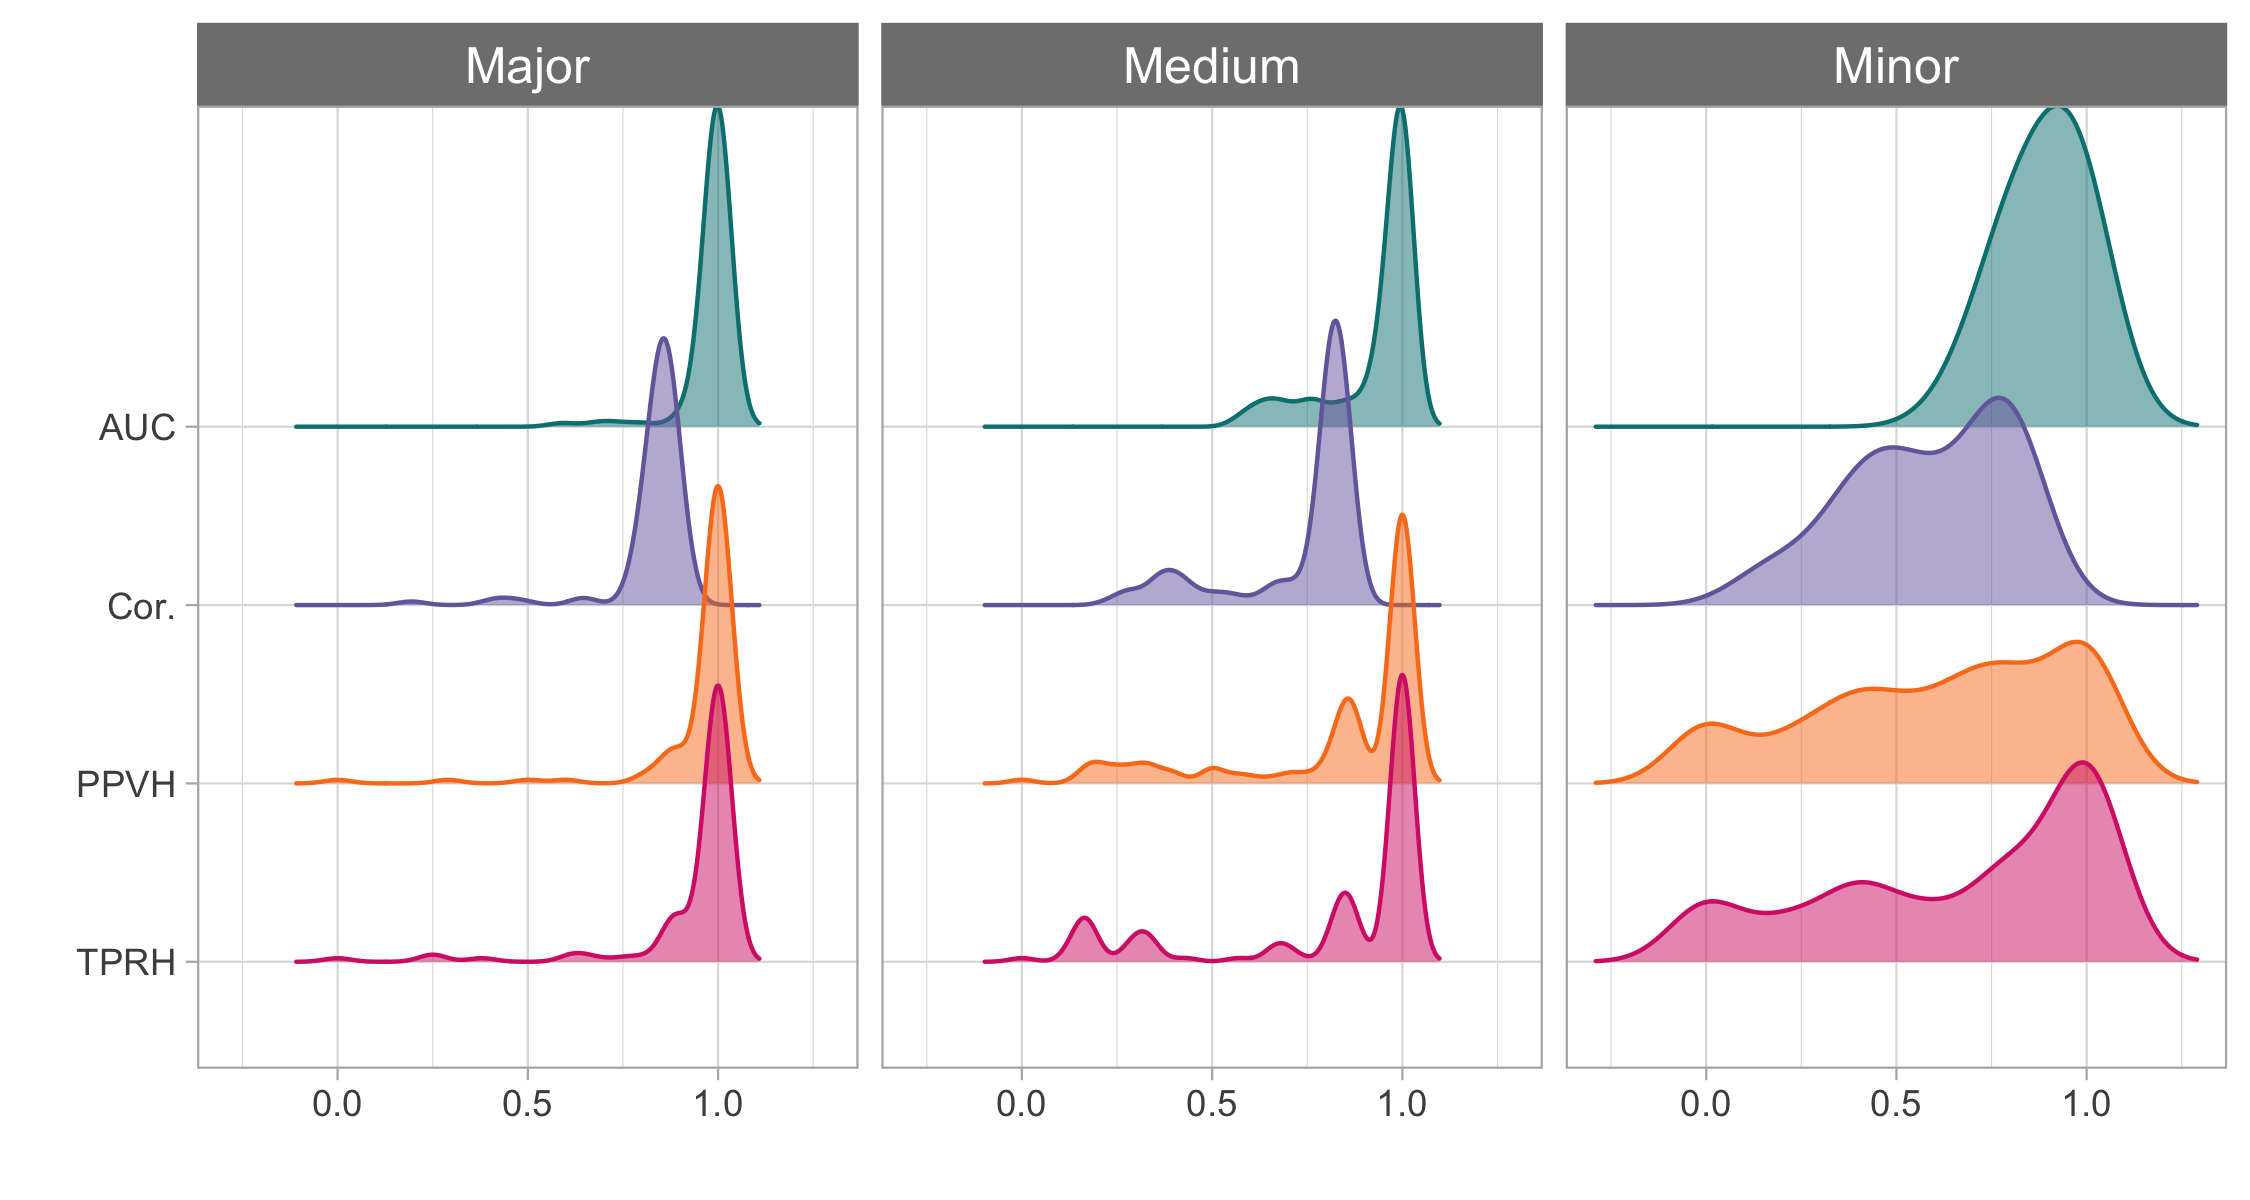
\includegraphics[width=11cm]{figs/simu_densities.png}
    \caption{
    %\CA{}
    The influence of the missing actor is measured with its degree, distinguishing three influence classes: \textit{Minor} (degree $\leq 5$), \textit{Medium} ($5<$ degree $\leq 7$) and \textit{Major} (degree $\geq 8$). 
    %\CA{Distributions of performance measures}
    The distributions of performance measures are displayed for each class of influence: AUC measures the retrieval of the dependence structure between all variables, observed and missing.  Precision and recall are specific to the missing actor links. 
    }
    \label{fig:densities}
\end{figure}
 

\begin{figure}[H]
    \centering    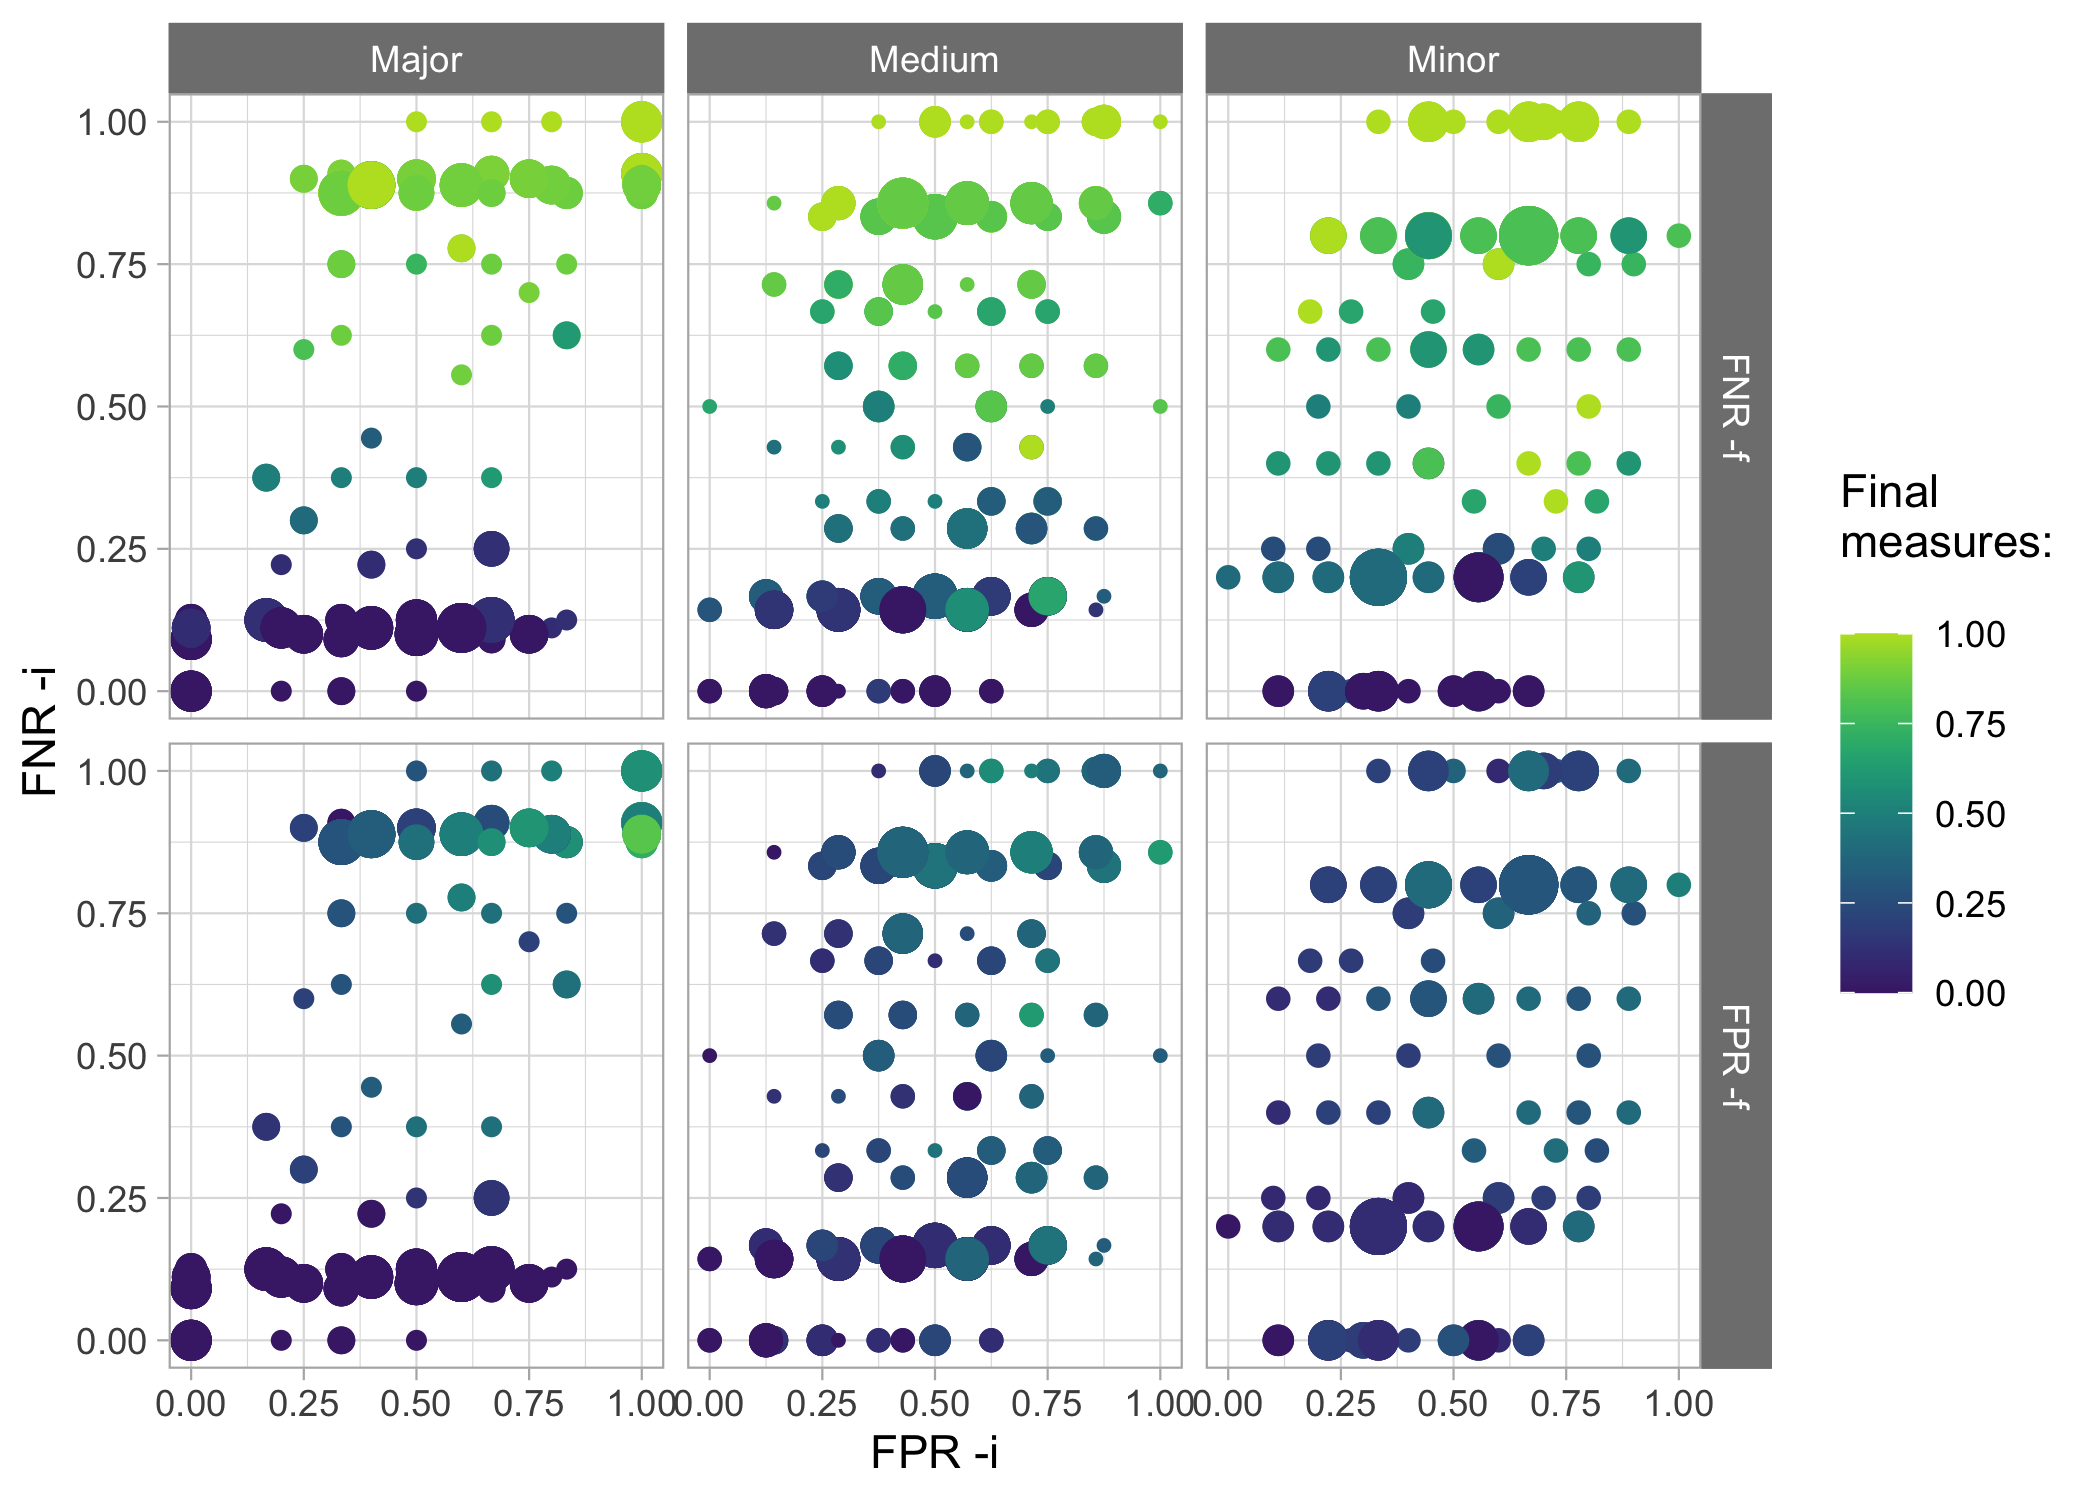
\includegraphics[width=11cm]{figs/quali_init_spca.png}
    \caption{Comparison of initial and final FPR and FNR, for cliques of neighbors of one missing actor obtained with the sparse PCA method. Position of dots are defined according to initial values, their color according to the final FPR and FNR. Sizes are proportional to the density of dots on a given position.}
    \label{fig:perfinit}
\end{figure}


 \begin{table}
\centering
\begin{tabular}{lrrrrrr}
  \hline
  & N & AUC & Precision & Recall & Cor. &t(s) \\ 
  \hline
  Major & 100 & 1 (0.00) & 1 (0.00) & 1 (0.01) & 0.86 (0.02)  & 1.28 (0.21) \\ 
  Medium & 132 & 1 (0.02) & 1 (0.00) & 0.99 (0.04) & 0.83 (0.02)  & 1.38 (0.46)  \\ 
  Minor &  68 & 0.98 (0.04) & 0.99 (0.03) & 0.96 (0.12) & 0.8 (0.04)& 1.56 (0.69) \\ 
   \hline
\end{tabular}
 \caption{\label{tab:oracle} Oracle procedure using true clique as starting point. The influence of the missing actor is measured with its degree, distinguishing three influence classes: \textit{Minor} (degree $\leq 5$), \textit{Medium} ($5<$ degree $\leq 7$) and \textit{Major} (degree $\geq 8$).  For each class of influence, the following quantities are reported:  number of simulated graphs (N), means and standard deviations of AUC, Precision, Recall, Correlation between missing actor inferred vector of means and original latent vector, and running times in seconds. AUC measures the retrieval of the dependence structure between all variables (observed and missing), whereas precision and recall are specific to the missing actor links.}
\end{table}
\section{Applications}  \label{sec:Appli}


%%%%%%%%%%%%%%%%%%%%%%%%%%%%%%%%%%%%%%%%%%%%%%%%%%%%%%%%%%%%%%
\subsection{Cross validation criterion for  model selection}
%\SR{
%As no model selection criteria has been designed for this problem yet, we  run a 10-fold cross-validation procedure, with pairwise composite likelihood (PCL) as adjustment criteria (see \citet{lindsay}). This choice of pairwise components is motivated from the fact that they keep track of the covariance structure, and the estimation of bivariate Poisson log-normal densities is made possible thanks to the \texttt{bipoilog} function of the \texttt{poilog} R package. \\
%
%The cross-validation procedure to estimate the pairwise composite likelihood is available in appendix \ref{CV}. The general idea is to compute the bivariate Poisson log-normal densities between all pair of species, conditional on a tree sampled as explained in appendix \ref{sampTrees} which defines the distribution parameters. Finally the procedure computes the average criteria  $$\displaystyle PCL(\Ybf)=\frac1V\sum_{v=1}^{V}\frac1B \sum_{b=1}^Bf_{PLN}(\Ybf; b,v),$$ where $f_{PLN}(\Ybf; b,v)=\sum_{\substack{i \in v\\ j < k}} \log p_{PLN}[(Y_{ij}^v, Y_{ik}^v) | T^b; \widehat{\theta},\widehat{\Sigma}_{T^b jk}]$, with $V=10$ and $B=10^2$. \\
%This is a computational greedy procedure that is not suited for a simulation study. It was applied to two empirical datasets in order to decide the number of missing actors in the model. The results, gathered in Figure \ref{fig:selec}, yield $r=1$ for the Barents Sea data set, and $r=2$ for the Fatala River one.}{}

The proposed model obviously raises the problem of choosing the number of missing actors $r$ (which may be zero). Variational-based inference often relies on approximate versions of the BIC or ICL criteria for model selection. Few theoretical guaranties exist about these approximate criteria and, in the present case, we observed that BIC and ICL penalizations did not yield consistent results. Therefore, we resort to $V$-fold cross validation to determine the number of missing actors. 

More specifically, we split the original dataset $\Ybf$ ($\Xbf$ is dropped here for the sake of clarity) into $V$ subsets with almost equal sizes $m_1, \dots m_V$ ($\sum_{v=1}^V m_v = n$), which we denote $\{\Ybf^v\}_{v = 1, \dots V}$. For each subset $v$, we define its complement $\Ybf^{-v}$ on which we fit a model with $r$ missing actors and get a parameter estimate $\Gammabf_r^{-v} = (\thetabf_r^{-v}, \sigmabf_r^{-v}, \betabf^{-v}_r, \Omegabf_r^{-v})$ and measure the fit of $\Gammabf_r^{-v}$ to the test dataset $\Ybf^v$. 

To avoid the integration over the $(p+r)$-dimensional Gaussian latent layer, we measure the fit with the pairwise composite likelihood \citep{lindsay}.
For any given tree $T$ and parameter $\Gammabf$, the bivariate Poisson log-normal pdf $p_{PLN}\left((Y_{ij}, Y_{ik}); \Gammabf, T \right)$ can be easily computed for any sample $i$ and pair of species $(j, k)$ with available tools such as the \texttt{poilog} R package \citep{ViS08} available on CRAN. The cross-validation criterion is defined as
$$
PCL_r(\Ybf) = \frac1V \sum_v \frac1B \sum_{b=1}^B \frac1{m_v} \sum_{i = 1}^{m_v} \sum_{j < k} \log p_{PLN}\left((Y^v_{ij}, Y^v_{ik}); \Gammabf_r^{-v}, T_{r, b}^{-v} \right)
$$
where the tree samples $\{T_{r, b}^{-v}\}_{b=1 \dots B}$ are iid according to $p_{\betabf_r^{-v}}(T)$. 

The sampling procedure for spanning trees is given in Appendix \ref{eq:sampTree}; the complete procedure for the calculation of $PCL_r(\Ybf)$ is described by Algorithm \ref{algo:model-selection}, given in Appendix \ref{sec:modSel}. Note that this criterion measures the fit of the model in terms of abundance prediction, whereas our interest is mostly focused on the inference of the dependency structure. In other words, our goal is identification, that is selecting the smallest model  and not the best model in terms of prediction \citep{arlot2010survey}.


We did not include this computationally greedy procedure in the simulation study but applied it to the two ecological datasets that will be described in the next two sections. The results, gathered in Figure \ref{fig:selec}, yield $r=1$ missing actor for the Barents Sea data set, and $r=2$ missing actors for the Fatala River one.

\begin{figure}[H]
    \centering
    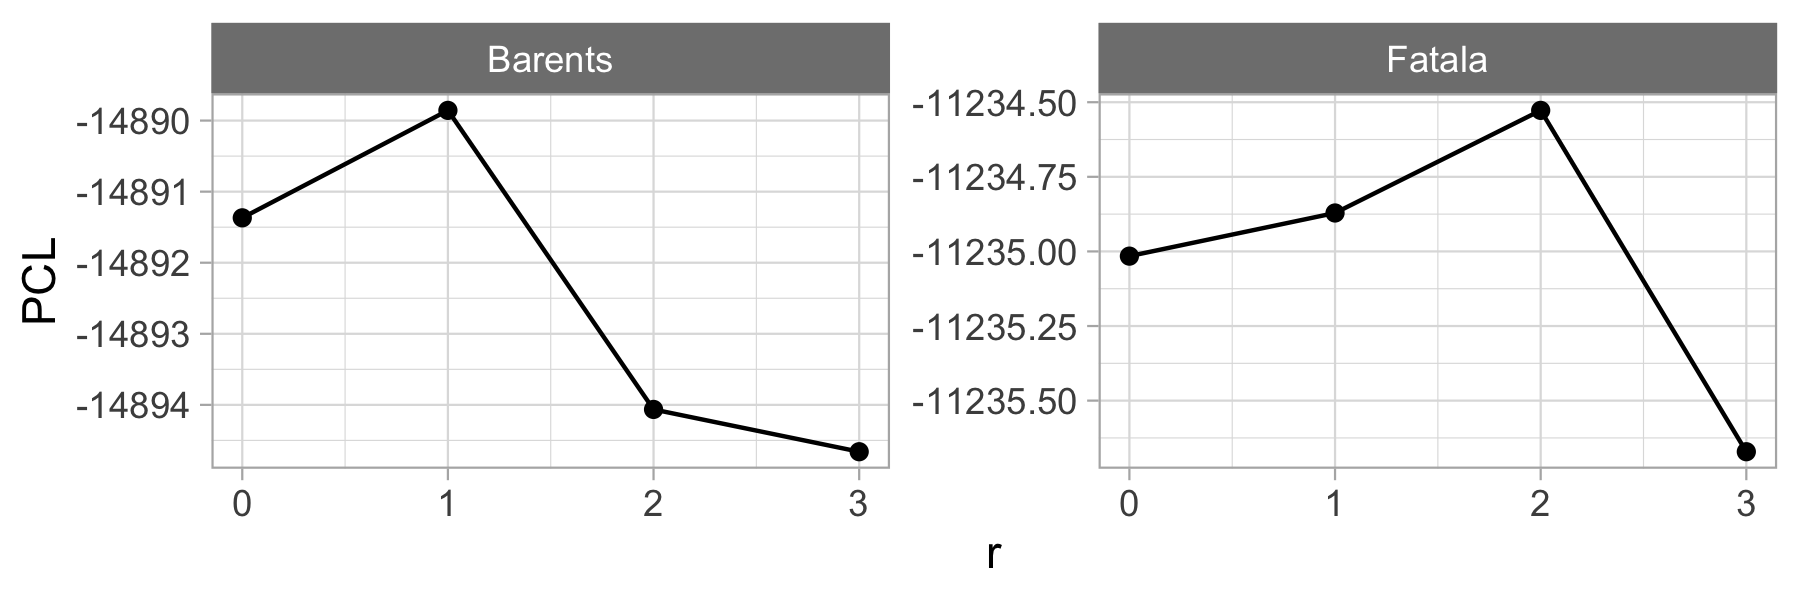
\includegraphics[width=10cm]{figs/selec_model_applis.png}
    \caption{Pairwise composite likelihoods estimates of Barents and Fatala datasets for models including 0 to 3 missing actors.}
    \label{fig:selec}
\end{figure}

% \SR{
% A wider exploration of likely cliques is conducted thanks to a bootstrap approach with $200$ sub-samples. Each of the latter consists of 80\% of the data; sPCA is run on each of them and only the identified clique of the $r$ first principal components are stored, when the studied model involves $r$ missing actors. When $r>1$, the restriction on the clique sizes is lifted. The bootstrap thus yield 200 lists of $r$ initial cliques, from which only unique ones are kept. This approach is more time-consuming, and therefore only used on empirical datasets.
% }{
Regarding the initialization, we performed a wider exploration as compared to the simulation study. To enlarge the list of possible cliques, we applied a resampling version of the procedure described in Section \ref{sec:algoSpec}, and applied it to 200 sub-samples, each consisting in 80\% of the whole data set. This yielded 200 lists of $r$ initial cliques, from which duplicates were removed.
%}

%%%%%%%%%%%%%%%%%%%%%%%%%%%%%%%%%%%%%%%%%%%%%%%%%%%%%%%%%%%%%%%%%%%%%%%%%%%%%%%%
\subsection{Barents Sea}
%data availability ? précisions sur les données, elles viennent d'où

% \SR{30 species of fish were counted in 89 sites of the Barents Sea (shrimp survey in the period April-May 1997, available at  \url{https://www.fbbva.es/microsite/multivariate-statistics/data.html})}{
The dataset was first published by \cite{FNA06} and consists of the abundance of 30 fish species measured in 89 sites in the Barents See in April-May 1997. In addition to abundances, the water temperature was measured in each site. The complete dataset is available at \url{www.fbbva.es/microsite/multivariate-statistics/data.html}. 
Fishes distributions are known to be greatly linked with the temperature. 
Hence to illustrate our methodology, 
% \SR{models were fit\CA{}{ted} without any covariates and with one missing actor, which we denote $h$. $\rm{Cor}(k,temp)$ denotes the absolute Pearson's correlation between $M_k$ (estimated vector of means of node $k$ along all 89 sites) and the temperature.}{
we present the results of the model fitted without any covariate (that is not accounting for the temperature), but including one missing actor (as suggested by Figure \ref{fig:selec}). To assess the ability of the proposed methodology to retrieve the influence of temperature as a missing actor, we report the empirical correlation between the temperature and the conditional expectation of the missing actor $M_h$, which we denote $\corHTemp$.
 
% Runing time
The resampling initialization procedure yielded in 14 different cliques, for each of which a VEM algorithm was run: the mean running time was $6.63$mins with deviation $0.70$ mins. 

% Dependency structure
The edge probabilities involving node $h$ as an endpoint were either very close to 0 or very close to 1, yielding a total of 6 highly probable neighbors of $h$. Figure \ref{fig:barents_adj} shows that many direct interactions are inferred between the corresponding 6 species in absence of a missing actor, which vanish when it is introduced. It also shows that accounting for this actor has only a local effect and that the direct interactions among the other species are preserved, which is consistent with our notion of a missing actor.

\begin{figure}[H]
    \centering
    \includegraphics[width=10cm]{figs/Barents_mat_comp.png} \\\vspace{-2cm}
    \includegraphics[width=10cm]{figs/Barents_net_comp3.png}
    \caption{\textit{Top left:} adjacency matrix of the Barents Sea fishes interaction network for $r=0$  missing actor. The inferred neighbors are gathered in the last 6 columns, so that their interactions are observable in the upper-right corner. \textit{Top right:} adjacency matrix for $r=1$  missing actor. The last column gathers the interactions of the inferred missing actor. \textit{Bottom}: Inferred interaction network with $r=0$ (left) and $r=1$ (right). Colored nodes refer to the inferred neighbors (blue) of the missing actor (yellow). The edges width are proportional to their probability.}
    \label{fig:barents_adj}
\end{figure}

%\begin{figure}[H]
%    \centering
%    \includegraphics[width=10cm]{missing_article/Fig/Barents_net_comp3.png}
%    \caption{Barents Sea fishes interaction network with $r=0$ (left) and $r=1$ (right). Colored nodes refer to the inferred neighbors (blue) of the missing actor (yellow).}
%    \label{fig:barents_net}
%\end{figure}

% Interpretation
In terms of interpretation, Figure \ref{fig:barents_temp} shows that the missing actor is highly correlated with the temperature. It also appears that the abundances of the species neighbor to the missing actor are much more correlated with the temperature (mean correlation = 0.78, sd = .06) than the abundances of the non-neighbor species (mean correlation = 0.46, sd = .27). This example shows the ability of the method to recover an underlying effect that would not be recorded in the data.

\begin{figure}
    \centering
    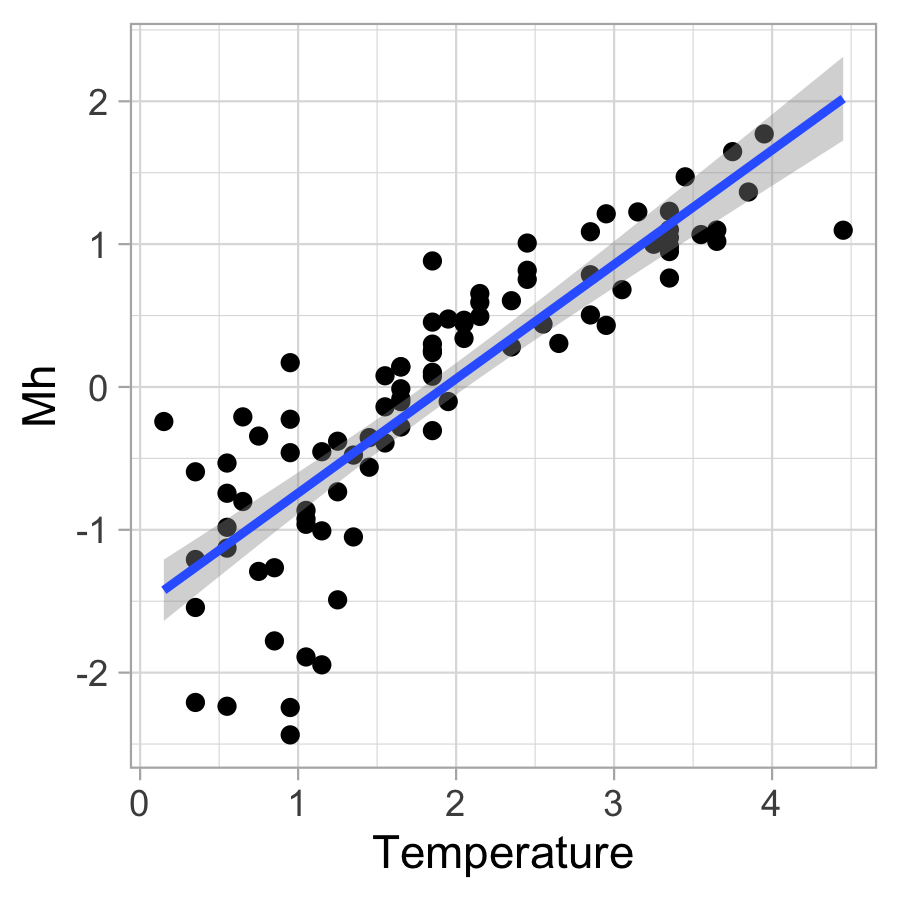
\includegraphics[width=5cm]{figs/Barents_MH_temp_white.png}
    \caption{Missing actor estimated vector of means $M_h$ as a function of the temperature. $\corHTemp=0.85$.}
    \label{fig:barents_temp}
\end{figure}

% \SR{
% Table \ref{tab:barents} then gathers the mean of correlations to the temperature of neighbors and non-neighbors. It appears that neighbors to the missing actor are significantly more correlated to the temperature than other nodes are.
% \begin{table}[ht]
% \centering
% \begin{tabular}{rlrr}
%   \hline
%   $P_{hk}$ & $\corKTemp$  \\ 
%   \hline
%  $<0.5$  & 0.44 (0.25)\\ 
%   $\geq 0.5$ & 0.80 (0.06) \\ 
%   \hline
% \end{tabular}
% \caption{Mean and standard deviation of $\corKTemp$ in relation with node $k$ being inferred as a neighbor ($P_{hk}\geq 0.5$) of missing actor $h$ or not ($P_{hk}< 0.5$).}
% \label{tab:barents}
% \end{table}
% }{
%} 

%\begin{figure}
%    \centering
%    \includegraphics[width=9cm]{missing_article/Fig/Barents_mat_comp.png}
%    \caption{\textit{Left:} adjacency matrix of Barents Sea fishes interaction network for $r=0$. The inferred neighbors are gathered in the last 6 columns, so that their interactions are observable in the upper-right corner. \textit{Right:} adjacency matrix of Barents Sea fishes interaction network for $r=1$. The last column gathers the interactions of the inferred missing actor.}
%    \label{fig:my_label}
%\end{figure}

%\begin{figure}[H]
%    \centering
%    \includegraphics[width=10cm]{missing_article/Fig/Barents_net_comp3.png}
%    \caption{Barents Sea fishes interaction network with $r=0$ (left) and $r=1$ (right). Colored nodes refer to the inferred neighbors (blue) of the missing actor (yellow).}
%    \label{fig:my_label}
%\end{figure}

%%%%%%%%%%%%%%%%%%%%%%%%%%%%%%%%%%%%%%%%%%%%%%%%%%%%%%%%%%%%%%%%%%%%%%%%%%%%%%%%
\subsection{Fatala River}
% \SR{
% The R package \texttt{ade4}  provides with the baran95 dataset which gathers the abundances of 33 species of fish on 90 locations of the Fatala River in Guinea. Data sampled between June 1993 and February 1994, which we organize in dry and rainy seasons; dates and sites are available as dataset categorical covariates.
% %
% Again models are fit with no covariates, and here two missing actors are inferred, which we denote $h1$ and $h2$. As models include more than one missing actor, the best VEM is selected under the constraint $\log sd(M_h)\geq -20$ for $h\in \{h1, h2\}$. This constraint ensures that the corresponding marginal variance of each missing actor is not too high, which would mean that the algorithm did not learn a lot about them. In other words, this ensures the algorithm succeeds in finding the desired number of missing actors. \\
% %
% The bootstrap method gives 60 unique  lists of two possible initial cliques and the mean running time for a convergence with precision $1e-3$ is $11.33$ min with deviation $1.47$; 14 did not reach convergence and the algorithm stopped after 100 iterations. \\
% %
% The best fit gives vectors of means $Mh1$ and $Mh2$ corresponding two each missing actor. Figure \ref{fig:Fatala} shows the plot of $Mh1$ against $Mh2$ colored with either one of the available covariates. It is very interesting to see that $Mh1$ is linked to the Site covariate, as it clearly separates kilometer 3 from kilometer 46 which are the first and last locations. On the other hand $Mh2$ seems linked with the Season covariate, even if the separation is less obvious.
% }{
\cite{baran1995dynamique} collected the abundances of 33 fish species in 90 sites along the Fatala River in Guinea between June 1993 and February 1994. The data are available from the R package \texttt{ade4} on CRAN \citep{dray2007ade4}, along with the date and site of collection, from which we deduce the season (dry or rainy). Again the model was fitted without any covariates, but with two missing actors, as suggested by Figure \ref{fig:selec}. \\
%
The resampling initialization procedure yielded in 60 different cliques, for each of which a VEM algorithm was run: the mean running time was $11.33$ min (sd = $1.47$ mn). 14 VEM did not reach convergence (with tolerance $\varepsilon = 1e-3$) after 100 iterations. We filtered out the results obtained from the different initializations, when the algorithm obviously ended in a degenerate solution ($\Var(M_h) < \exp(-20)$). \\ 
%
% %\SR{
% Figure \ref{fig:Fatala} shows the scatterplot of estimated conditional mean of the two missing actors $(M_{h_1}, M_{h_2})$ in each site, colored with either one of the available covariates (site and season). $M_{h_1}$ is obviously linked to the site and separates most upstream locations (kilometer 3) from most downstream locations (kilometer 46). On the other hand $M_{h_2}$ seems linked with the Season covariate, even if the separation is less obvious. Similarly, the second missing actor shows a clear relation with the season. \\
% % 
% Again, the retrieved missing actor each correspond to an underlying effect that rules fish species abundances. The clear separation between the two effects is reinforced by the assumption the missing actors are independent from each other, which obviously holds for locations ans seasons. \\
% }{
Figure \ref{fig:Fatala} shows the scatterplot of the estimated conditional mean of the two missing actors $(M_{h_1}, M_{h_2})$ in each site, colored with either one of the available covariates (site and season). The missing actor $h_1$ is obviously linked to the site and separates most upstream locations (kilometer 3) from most downstream locations (kilometer 46). This actor has 11 highly probable neighbor species.
% \textcolor{red}{comparer les anova Poisson pour les voisins / pas voisins}
Again, this retrieved missing actor corresponds to an underlying effect (in this case: geography) that rules fish species abundances. \\
% 
The second missing actor seems to be linked with the season but with a less clear separation. Also the variability of $M_{h_2}$ is much smaller than this of $M_{h_1}$. This effect is therefore questionable, which brings us back to model selection. As mentioned above, we used a procedure based on cross-validation, which may  be prone to select too complex model \citep{shao1993linear,friedman2001elements,arlot2010survey}. The definition of a grounded model selection criterion for structure inference in presence of missing actors remains open.
%}

%\textcolor{red}{[C'est un peu dommage de finir comme ça mais bon...]}
 
\begin{figure}[h]
    \centering
    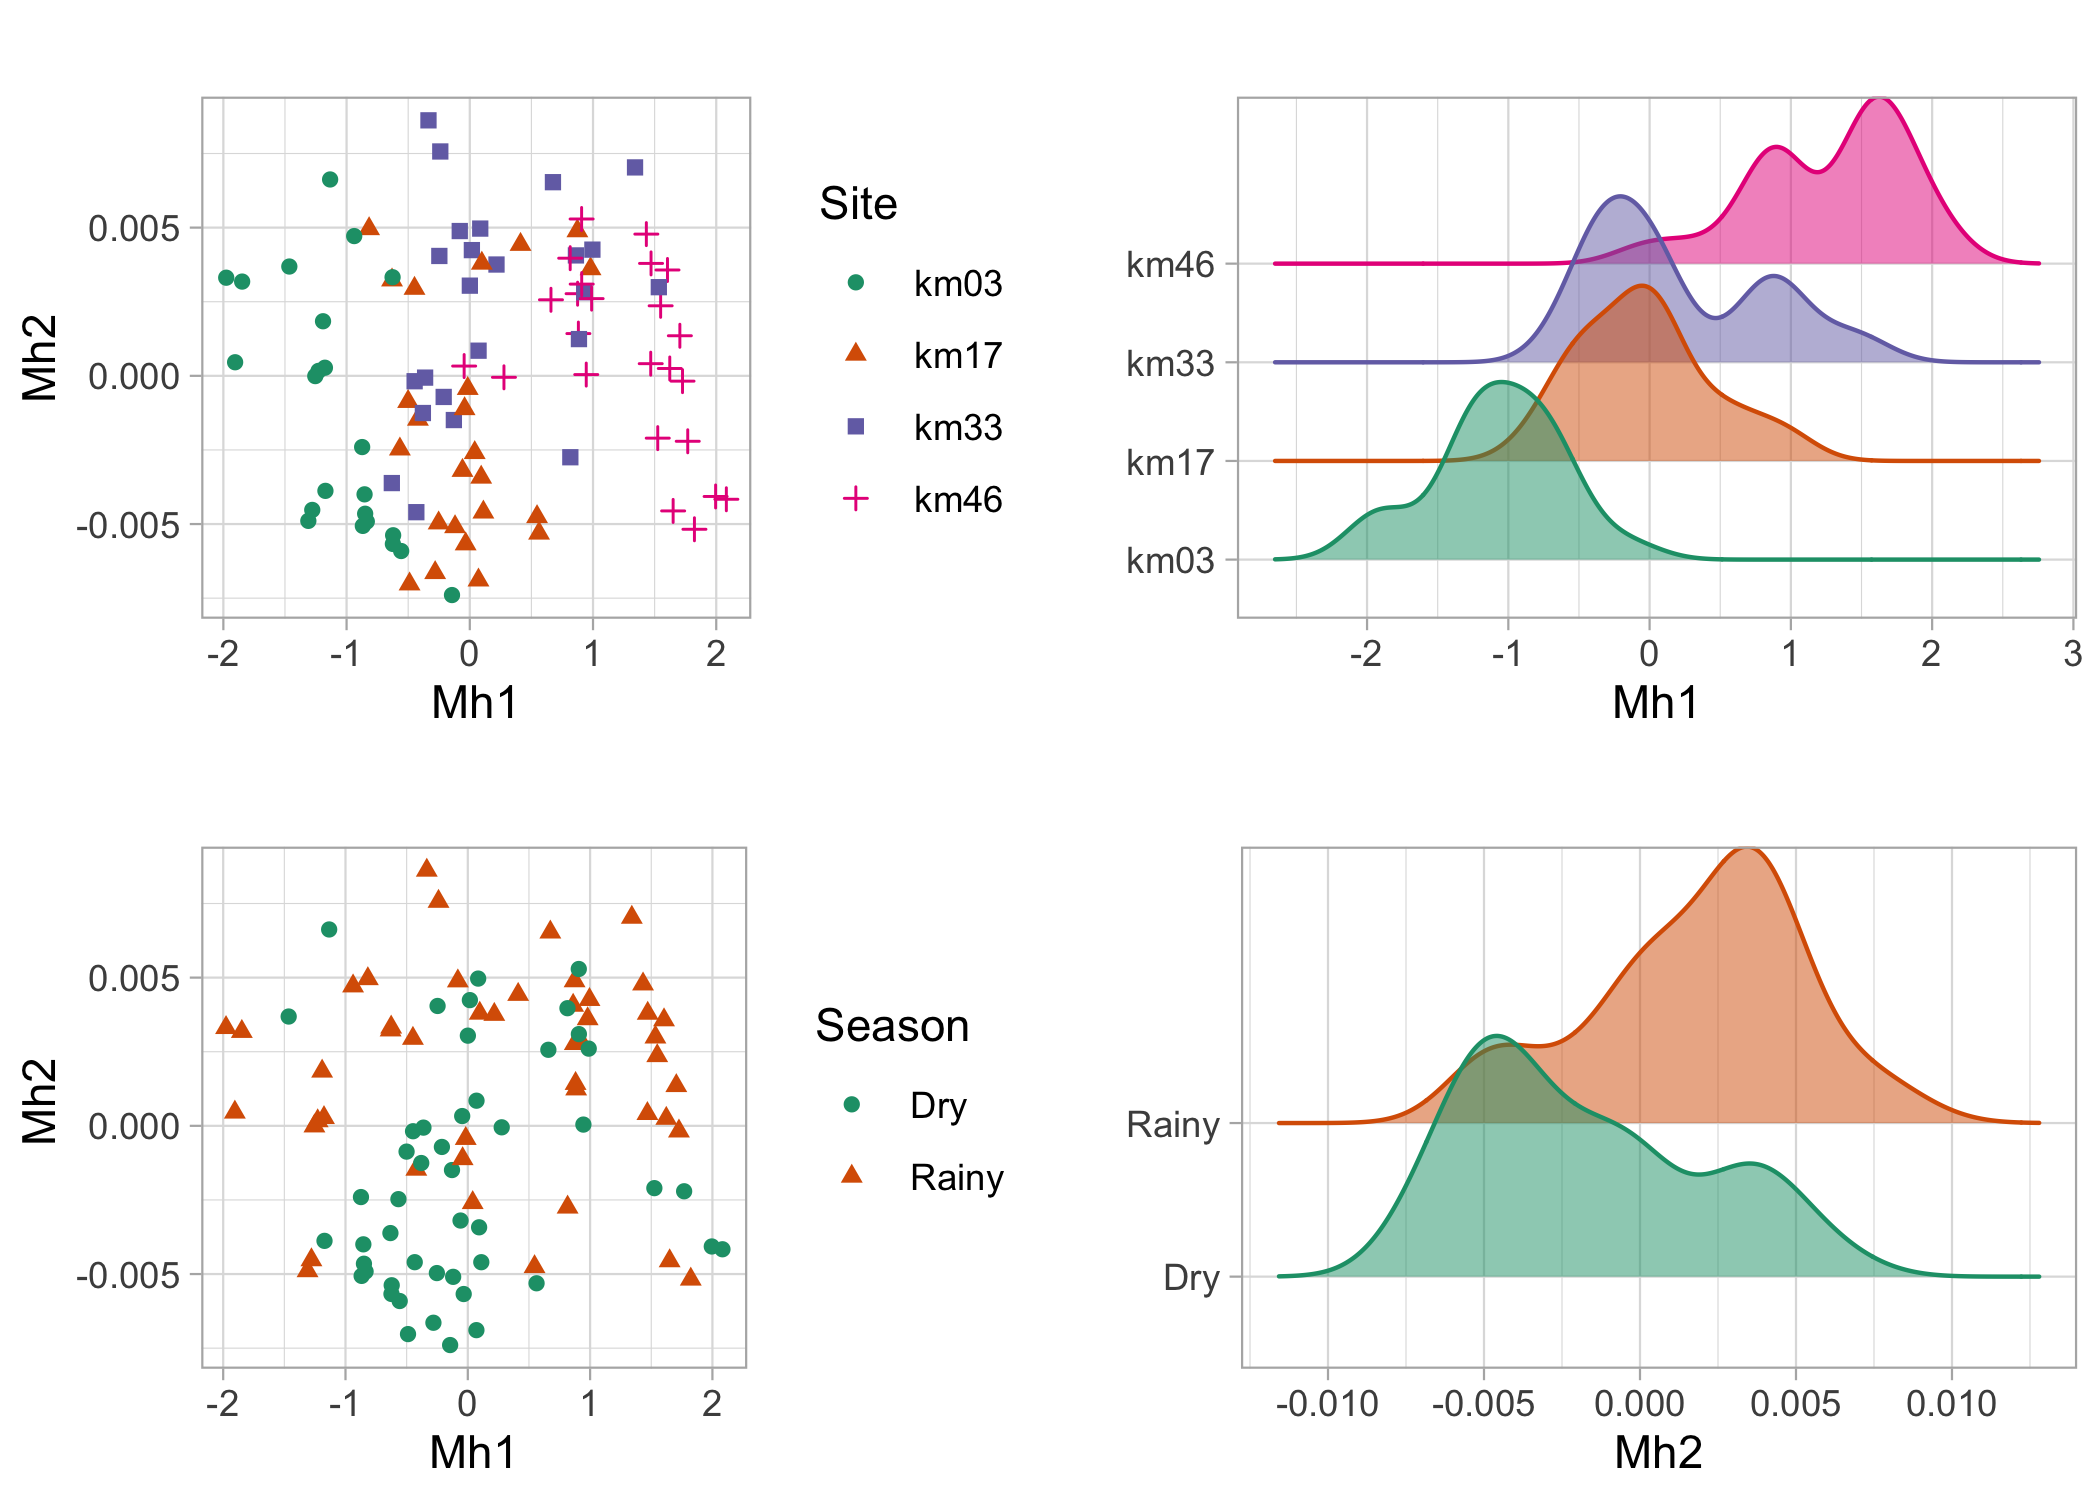
\includegraphics[width=12cm]{figs/Fatala_MH2.png}
    \caption{Estimated means $M_{h_1}$ and $M_{h_2}$ of the two inferred missing actors. Left column: scatterplots $M_{h_1}$ vs $M_{h_2}$ with site (top) and season (bottom) color code. Right: distribution of the estimated means across sites. Top right: distribution of $M_{h_1}$ in each location, bottom right: distribution of $M_{h_2}$ in each season.}
    \label{fig:Fatala}
\end{figure}



%\input{normalizedModel}
%\input{intro_old.tex}
%\input{model_old.tex}
%\input{inference_old.tex}


\paragraph{Acknowledgements.} 
This work was partly supported by the French ANR-18-CE02-0010 Ecological Networks (EcoNet) project and by the French ANR-11-LABX-0056-LMH LabEx Laboratoire de Mathématique Hadamard.
\begin{thebibliography}{}

\bibitem[\protect\citeauthoryear{Aitchison and Ho}{Aitchison and
  Ho}{1989}]{AiH89}
Aitchison, J. and C.~Ho (1989).
\newblock The multivariate {P}oisson-log normal distribution.
\newblock {\em Biometrika\/}~{\em 76\/}(4), 643--653.

\bibitem[\protect\citeauthoryear{Ambroise, Chiquet, and Matias}{Ambroise
  et~al.}{2009}]{ambroise2009inferring}
Ambroise, C., J.~Chiquet, and C.~Matias (2009).
\newblock Inferring sparse gaussian graphical models with latent structure.
\newblock {\em Electronic Journal of Statistics\/}~{\em 3}, 205--238.

\bibitem[\protect\citeauthoryear{Arlot and Celisse}{Arlot and
  Celisse}{2010}]{arlot2010survey}
Arlot, S. and A.~Celisse (2010).
\newblock A survey of cross-validation procedures for model selection.
\newblock {\em Statistics surveys\/}~{\em 4}, 40--79.

\bibitem[\protect\citeauthoryear{Baran}{Baran}{1995}]{baran1995dynamique}
Baran, E. (1995).
\newblock {\em Dynamique spatio-temporelle des peuplements de Poissons
  estuariens en Guin{\'e}e (Afrique de l'Ouest)}.
\newblock Ph.\ D. thesis, Th{\`e}se de Doctorat, Universit{\'e} de Bretagne
  Occidentale.

\bibitem[\protect\citeauthoryear{{Blei}, {Kucukelbir}, and {McAuliffe}}{{Blei}
  et~al.}{2017}]{BKM17}
{Blei}, D.~M., A.~{Kucukelbir}, and J.~D. {McAuliffe} (2017).
\newblock Variational inference: A review for statisticians.
\newblock {\em Journal of the American Statistical Association\/}~{\em
  112\/}(518), 859--877.

\bibitem[\protect\citeauthoryear{Cand{\`e}s, Li, Ma, and Wright}{Cand{\`e}s
  et~al.}{2011}]{candes2011robust}
Cand{\`e}s, E., X.~Li, Y.~Ma, and J.~Wright (2011).
\newblock Robust principal component analysis?
\newblock {\em Journal of the ACM (JACM)\/}~{\em 58\/}(3), 1--37.

\bibitem[\protect\citeauthoryear{Chaiken and Kleitman}{Chaiken and
  Kleitman}{1978}]{matrixtree}
Chaiken, S. and D.~J. Kleitman (1978).
\newblock Matrix tree theorems.
\newblock {\em Journal of combinatorial theory, Series A\/}~{\em 24\/}(3),
  377--381.

\bibitem[\protect\citeauthoryear{Chandrasekaran, Sanghavi, Parrilo, and
  Willsky}{Chandrasekaran et~al.}{2011}]{RankSparse}
Chandrasekaran, V., S.~Sanghavi, P.~A. Parrilo, and A.~S. Willsky (2011).
\newblock Rank-sparsity incoherence for matrix decomposition.
\newblock {\em SIAM J. Optim\/}~{\em 21}, 572--596.

\bibitem[\protect\citeauthoryear{Chiquet, Mariadassou, and Robin}{Chiquet
  et~al.}{2018}]{CMR18}
Chiquet, J., M.~Mariadassou, and S.~Robin (2018).
\newblock Variational inference for probabilistic poisson pca.
\newblock {\em The Annals of Applied Statistics\/}~{\em 12\/}(4), 2674--2698.

\bibitem[\protect\citeauthoryear{Chiquet, Mariadassou, and Robin}{Chiquet
  et~al.}{2019}]{CMR19}
Chiquet, J., M.~Mariadassou, and S.~Robin (2019).
\newblock Variational inference for sparse network reconstruction from count
  data.
\newblock In {\em International Conference on Machine Learning}.

\bibitem[\protect\citeauthoryear{Chow and Liu}{Chow and Liu}{1968}]{ChowLiu}
Chow, C. and C.~Liu (1968, May).
\newblock Approximating discrete probability distributions with dependence
  trees.
\newblock {\em IEEE Transactions on Information Theory\/}~{\em 14\/}(3),
  462--467.

\bibitem[\protect\citeauthoryear{Dempster, Laird, and Rubin}{Dempster
  et~al.}{1977}]{DLR77}
Dempster, A.~P., N.~M. Laird, and D.~B. Rubin (1977).
\newblock Maximum likelihood from incomplete data via the {EM} algorithm.
\newblock {\em J. Royal Statist. Soc., series B\/}~{\em 39}, 1--38.

\bibitem[\protect\citeauthoryear{Devroye}{Devroye}{1986}]{Dev86}
Devroye, L. (1986).
\newblock {\em Non-uniform random variate generation}.
\newblock Springer.

\bibitem[\protect\citeauthoryear{Dray, Dufour, et~al.}{Dray
  et~al.}{2007}]{dray2007ade4}
Dray, S., A.-B. Dufour, et~al. (2007).
\newblock The ade4 package: implementing the duality diagram for ecologists.
\newblock {\em Journal of statistical software\/}~{\em 22\/}(4), 1--20.

\bibitem[\protect\citeauthoryear{Durfee, Kyng, Peebles, Rao, and
  Sachdeva}{Durfee et~al.}{2017}]{DKP17}
Durfee, D., R.~Kyng, J.~Peebles, A.~B. Rao, and S.~Sachdeva (2017).
\newblock Sampling random spanning trees faster than matrix multiplication.
\newblock In {\em Proceedings of the 49th Annual ACM SIGACT Symposium on Theory
  of Computing}, pp.\  730--742.

\bibitem[\protect\citeauthoryear{Erichson, Zheng, Manohar, Brunton, Kutz, and
  Aravkin}{Erichson et~al.}{2020}]{spca}
Erichson, N.~B., P.~Zheng, K.~Manohar, S.~L. Brunton, J.~N. Kutz, and A.~Y.
  Aravkin (2020).
\newblock Sparse principal component analysis via variable projection.
\newblock {\em SIAM Journal on Applied Mathematics\/}~{\em 80\/}(2), 977--1002.

\bibitem[\protect\citeauthoryear{Fossheim, Nilssen, and Aschan}{Fossheim
  et~al.}{2006}]{FNA06}
Fossheim, M., E.~M. Nilssen, and M.~Aschan (2006).
\newblock Fish assemblages in the {B}arents {S}ea.
\newblock {\em Marine Biology Research\/}~{\em 2\/}(4), 260--269.

\bibitem[\protect\citeauthoryear{Friedman, Hastie, and Tibshirani}{Friedman
  et~al.}{2001}]{friedman2001elements}
Friedman, J., T.~Hastie, and R.~Tibshirani (2001).
\newblock {\em The elements of statistical learning}, Volume~1.
\newblock Springer series in statistics New York.

\bibitem[\protect\citeauthoryear{Friedman, Hastie, and Tibshirani}{Friedman
  et~al.}{2008}]{FHT08}
Friedman, J., T.~Hastie, and R.~Tibshirani (2008).
\newblock Sparse inverse covariance estimation with the graphical lasso.
\newblock {\em Biostatistics\/}~{\em 9\/}(3), 432--441.

\bibitem[\protect\citeauthoryear{Giraud and Tsybakov}{Giraud and
  Tsybakov}{2012}]{GirLatent}
Giraud, C. and A.~Tsybakov (2012).
\newblock Discussion of "latent variable graphical model selection via convex
  optimization".
\newblock {\em Annals of Statistics\/}~{\em 40\/}(4), 1984--1988.

\bibitem[\protect\citeauthoryear{Inouye, Yang, Allen, and Ravikumar}{Inouye
  et~al.}{2017}]{inouye}
Inouye, D.~I., E.~Yang, G.~I. Allen, and P.~Ravikumar (2017).
\newblock A review of multivariate distributions for count data derived from
  the poisson distribution.
\newblock {\em Wiley Interdisciplinary Reviews: Computational
  Statistics\/}~{\em 9\/}(3), e1398.

\bibitem[\protect\citeauthoryear{Kirshner}{Kirshner}{2008}]{kirshner}
Kirshner, S. (2008).
\newblock Learning with tree-averaged densities and distributions.
\newblock In {\em Advances in Neural Information Processing Systems}, pp.\
  761--768.

\bibitem[\protect\citeauthoryear{Lauritzen and Meinshausen}{Lauritzen and
  Meinshausen}{2012}]{EMlvggm}
Lauritzen, S. and N.~Meinshausen (2012).
\newblock Discussion: Latent variable graphical model selection via convex
  optimization.
\newblock {\em The Annals of Statistics\/}~{\em 40\/}(4), 1973--1977.

\bibitem[\protect\citeauthoryear{Lauritzen}{Lauritzen}{1996}]{Lau96}
Lauritzen, S.~L. (1996).
\newblock {\em Graphical Models}.
\newblock Oxford Statistical Science Series. Clarendon Press.

\bibitem[\protect\citeauthoryear{Lindsay}{Lindsay}{1988}]{lindsay}
Lindsay, B.~G. (1988).
\newblock Composite likelihood methods.
\newblock {\em Contemporary mathematics\/}~{\em 80\/}(1), 221--239.

\bibitem[\protect\citeauthoryear{Lucas, Scholz, Boehme, Jasson, and
  Maechler}{Lucas et~al.}{2020}]{lucas2020package}
Lucas, A., I.~Scholz, R.~Boehme, S.~Jasson, and M.~Maechler (2020).
\newblock gmp: Multiple precision arithmetic.
\newblock R package version 0.5-13.6.

\bibitem[\protect\citeauthoryear{McLachlan and Krishnan}{McLachlan and
  Krishnan}{2007}]{mclachlan}
McLachlan, G. and T.~Krishnan (2007).
\newblock {\em The EM algorithm and extensions}, Volume 382.
\newblock John Wiley \& Sons.

\bibitem[\protect\citeauthoryear{Meil{\u{a}} and Jaakkola}{Meil{\u{a}} and
  Jaakkola}{2006}]{MeilaJaak}
Meil{\u{a}}, M. and T.~Jaakkola (2006).
\newblock Tractable bayesian learning of tree belief networks.
\newblock {\em Statistics and Computing\/}~{\em 16\/}(1), 77--92.

\bibitem[\protect\citeauthoryear{Meil{\u{a}} and Jordan}{Meil{\u{a}} and
  Jordan}{2000}]{MixtTrees}
Meil{\u{a}}, M. and M.~I. Jordan (2000).
\newblock Learning with mixtures of trees.
\newblock {\em Journal of Machine Learning Research\/}~{\em 1}, 1--48.

\bibitem[\protect\citeauthoryear{Meng, Eriksson, and III}{Meng
  et~al.}{2014}]{LLVGGM}
Meng, Z., B.~Eriksson, and A.~O.~H. III (2014).
\newblock Learning latent variable gaussian graphical models.
\newblock {\em Proceedings of the 31 International Conference on Machine
  Learning\/}~{\em 32}, 1269--1277.

\bibitem[\protect\citeauthoryear{Momal, Robin, and Ambroise}{Momal
  et~al.}{2020}]{MRA20}
Momal, R., S.~Robin, and C.~Ambroise (2020).
\newblock Tree-based inference of species interaction networks from abundance
  data.
\newblock {\em Methods in Ecology and Evolution\/}~{\em 11}, 621--632.

\bibitem[\protect\citeauthoryear{Popovic, Hui, and Warton}{Popovic
  et~al.}{2018}]{PHW18}
Popovic, G.~C., F.~K. Hui, and D.~I. Warton (2018).
\newblock A general algorithm for covariance modeling of discrete data.
\newblock {\em Journal of Multivariate Analysis\/}~{\em 165}, 86--100.

\bibitem[\protect\citeauthoryear{Popovic, Warton, Thomson, Hui, and
  Moles}{Popovic et~al.}{2019}]{PWT19}
Popovic, G.~C., D.~I. Warton, F.~J. Thomson, F.~K.~C. Hui, and A.~T. Moles
  (2019).
\newblock Untangling direct species associations from indirect mediator species
  effects with graphical models.
\newblock {\em Methods in Ecology and Evolution\/}~{\em 10\/}(9), 1571--1583.

\bibitem[\protect\citeauthoryear{Robin, Ambroise, and Robin}{Robin
  et~al.}{2019}]{RAR19}
Robin, G., C.~Ambroise, and S.~Robin (2019).
\newblock Incomplete graphical model inference via latent tree aggregation.
\newblock {\em Statistical Modelling\/}~{\em 19\/}(5), 545--568.

\bibitem[\protect\citeauthoryear{Schwaller and Robin}{Schwaller and
  Robin}{2017}]{ScR17}
Schwaller, L. and S.~Robin (2017).
\newblock Exact bayesian inference for off-line change-point detection in
  tree-structured graphical models.
\newblock {\em Statistics and Computing\/}~{\em 27\/}(5), 1331--1345.

\bibitem[\protect\citeauthoryear{{Schwaller}, {Robin}, and
  {Stumpf}}{{Schwaller} et~al.}{2019}]{SRS19}
{Schwaller}, L., S.~{Robin}, and M.~{Stumpf} (2019).
\newblock {Bayesian Inference of Graphical Model Structures Using Trees}.
\newblock {\em J. Soc. Franc. Stat.\/}~{\em 160\/}(2), 1--23.

\bibitem[\protect\citeauthoryear{Shao}{Shao}{1993}]{shao1993linear}
Shao, J. (1993).
\newblock Linear model selection by cross-validation.
\newblock {\em Journal of the American statistical Association\/}~{\em
  88\/}(422), 486--494.

\bibitem[\protect\citeauthoryear{Vidar and Steinar}{Vidar and
  Steinar}{2008}]{ViS08}
Vidar, G. and E.~Steinar (2008).
\newblock poilog: {P}oisson lognormal and bivariate {P}oisson lognormal
  distribution.
\newblock R package version 0.4.

\bibitem[\protect\citeauthoryear{Wainwright and Jordan}{Wainwright and
  Jordan}{2008}]{WaJ08}
Wainwright, M.~J. and M.~I. Jordan (2008).
\newblock Graphical models, exponential families, and variational inference.
\newblock {\em Found. Trends Mach. Learn.\/}~{\em 1\/}(1--2), 1--305.

\bibitem[\protect\citeauthoryear{Warton, Blanchet, O'Hara, Ovaskainen,
  Taskinen, Walker, and Hui}{Warton et~al.}{2015}]{WBO15}
Warton, D.~I., F.~G. Blanchet, R.~B. O'Hara, O.~Ovaskainen, S.~Taskinen, S.~C.
  Walker, and F.~K. Hui (2015).
\newblock So many variables: joint modeling in community ecology.
\newblock {\em Trends in Ecology \& Evolution\/}~{\em 30\/}(12), 766--779.

\bibitem[\protect\citeauthoryear{Zhao, Liu, Roeder, Lafferty, and
  Wasserman}{Zhao et~al.}{2012}]{zhao2012huge}
Zhao, T., H.~Liu, K.~Roeder, J.~Lafferty, and L.~Wasserman (2012).
\newblock The huge package for high-dimensional undirected graph estimation in
  r.
\newblock {\em The Journal of Machine Learning Research\/}~{\em 13\/}(1),
  1059--1062.

\end{thebibliography}


\begin{appendix}
\tocless \subsection{Algebraic Tools} \label{app:tools}
 We here present some algebraic results about spanning tree structures which are used during the computations. Theorem \ref{thm:MTT}, Lemma \ref{lem:Meila} as well as Lemma \ref{lem:Kirshner} use the notion of Laplacian matrix  $\Qbf$ of a symmetric matrix $\Wbf=[w_{jk} ]_{1\leq j,k\leq p}$, which is defined as follows :
 
\[
 [\Qbf]_{jk}  =\begin{cases}
    -w_{jk}  & 1\leq j<k \leq p\\
    \sum_{u=1}^p w_{ju} & 1\leq j=k \leq p.
    \end{cases}
\]
 
We further denote $\Wbf^{uv}$ the matrix $\Wbf$ deprived from its $u$th row and $v$th column and we remind that the $(u, v)$-minor of $\Wbf$ is the determinant of this deprived matrix, that is $|\Wbf^{uv}|$.
The following Theorem \ref{thm:MTT} is the extension of Kirchhoff's Theorem to the case of weighted graphs \citep{matrixtree,MeilaJaak}.\\
\begin{theorem}[Matrix Tree Theorem] \label{thm:MTT}
    For any symmetric weight matrix W with all positive entries, the sum over all spanning trees of the product of the weights of their edges is equal to any minor of its Laplacian. That is, for any $1 \leq u, v \leq p$,
   \[
    W := \sum_{T\in\mathcal{T}} \prod_{(j, k)\in T} w_{jk} = |\Qbf^{uv}|.
    \]\\
\end{theorem}    

In the following, without loss of generality, we will choose $\Qbf^{11}$. As an extension of this result, \cite{MeilaJaak} provide a close form expression for the derivative of $W$ with respect to each entry of $\Wbf$. 

\begin{lemma} [\cite{MeilaJaak}] \label{lem:Meila}
    Define the entries of the symmetric matrix $\Mbf$ as
 \[    
 [\Mbf]_{jk} =\begin{cases}
    \left[(\Qbf^{11})^{-1}\right]_{jj} + \left[(\Qbf^{11})^{-1}\right]_{kk} -2\left[(\Qbf^{11})^{-1}\right]_{jk} & 1< j<k \leq p\\
    \left[(\Qbf^{11})^{-1}\right]_{jj} & k=1, 1< j \leq p  \\
    0 &  j=k .
    \end{cases}
\]
it then holds that $$\partial_{w_{jk}} W = [\Mbf]_{jk}  \times W.$$\\
\end{lemma}

\cite{kirshner} build on Lemma \ref{lem:Meila} to provide an efficient computation of all edges probabilities.
\begin{lemma} [\cite{kirshner}] \label{lem:Kirshner}
    Let $p_W$ be a distribution on the space of spanning trees, such that $p_W(T)=\prod_{kl\in T} w_{kl} / W$, where $W$ is defined as in Theorem \ref{thm:MTT}. Taking the symmetric matrix $\Mbf$ as defined in Lemma  \ref{lem:Meila}, the probability for an edge $kl$ to be in the tree $T^*$ writes:
 
$$\mathds{P}\{kl\in T^*\} = \sum_{T\in \mathcal{T}} p_W(T)= w_{kl}\: \Mbf_{kl}$$
\end{lemma}


 \newpage

\tocless\subsection{Computations} \label{app:comput}
\subsubsection[Update of tree parameter vector]{Update of $\betabf$.} \label{up:beta}
As in \citet{MRA20}, the update of $\betabf$ is such that:
$$\betabf^{t+1}  = \arg\max_\betabf \; \Esp_{g^t} \left[ \log p_\betabf(T) \right].
$$
By definition of $p_\betabf(T)$:
$$\Esp_{g^t} \left[ \log p_\betabf(T) \right] = \sum_{kl} P^t_{kl} \log \beta_{kl} - \log B\;,
\qquad
B=\sum_{T\in \mathcal{T}}\prod_{kl\in T} \beta_{kl}.$$
Computing the derivative with respect to the edge weight $\beta_{kl}$ gives:
\begin{align*}
\partial_{\beta_{kl}}\Esp_{g^t} \left[ \log p_\betabf(T) \right] &=\frac{P_{kl}^t}{\beta_{kl}} - \frac{\partial_{\beta_{kl}} B^t }{B^t}.
\end{align*}
According to Lemma \ref{lem:Meila}: $\partial_{\beta_{kl}} B^t  = [\boldsymbol{M}]_{kl} \times B$. Finally setting the derivative to 0 yields the update formula $
\beta^{t+1}_{kl} 
= \frac{P^t_{kl}}{ M(\betabf^t)_{kl}}$.

\subsubsection[Update of Gaussian tree precision matrix]{Update of $\Omega_T$} \label{up:omega}
The update of $\Omegabf_T$ respects
$$\Omegabf^{t+1}  = \arg\max_\Omegabf \; \Esp_{q^t} \left[ \log p_{\Omegabf}(\Ubf \mid T) \right].$$
This is a problem of parameter optimisation in the context of Gaussian Graphical Models (GGM).
In what follows, for any $q\times q$  matrix $A$, $A_{[kl]}$ will refer to the block $kl$ of $A$: $A_{[kl]}=(a_{ij})_{\{i,j\}\in\{k,l\}}$.   $[A_{[kl]}]^q$ will then denote the matrix obtained by filling up with zero entries to obtain full dimension $q\times q$, so that:
$$([A_{[kl]}]^q )_{ij}=\left\{ \begin{array}{rl}
a_{ij} & \text{if } \{i,j\}\in\{k,l\}\\
0 &  \text{if } \{i,j\}\in\{1,..., q\}_{\setminus kl}
\end{array}\right.$$
In its proposition 5.9, \citet{Lau96} states that in a  GGM with $p$ variables and associated with the decomposable graph $\mathcal{G}$, the maximum likelihood of the precision matrix exists if and only if $n > \max_{C\in \mathcal{C}} |C|$. It is then given as 
$$\widehat{\Omega}=n\left(\sum_{C\in \mathcal{C}} [SSD_{[C]}\,^{-1}]^p - \sum_{S\in \mathcal{S}} \nu(S)\,[SSD_{[S]}\,^{-1}]^p \right)$$
where $\mathcal{C}$ is the set of cliques and $\mathcal{S}$ the set of separators of $\mathcal{G}$, with associated multiplicities $\nu(S)$.\\


In our context, $\mathcal{G}$ is a spanning tree and so all cliques are edges and separators are nodes. The multiplicity of a given node $k$ as a separator in the graph is  $\nu(k) = d(k)-1$, where $d(k)$ is its degree. Therefore the estimator  $\widehat{\Omega}_T$  writes as the following 
\begin{align*}
\widehat{\Omega}_T &= n  \sum_{kl\in T}   [(SSD_{[kl]})^{-1}]^{p+r} - n\sum_k (d(k)-1)[(SSD_{kk})^{-1}]^{p+r}\\
&=n \sum_{kl\in T}  [(SSD_{[kl]})^{-1} - (SSD_{kk})^{-1} -  (SSD_{ll})^{-1} ]^{p+r} + n\sum_k[(SSD_{kk})^{-1}]^{p+r}
\end{align*}
As $SSD$ has diagonal $n$, the expression simplifies. Denoting $I_d$ the identity matrix of dimension $d$ we obtain:
$$\widehat{\Omega}_T =n\sum_{kl\in T} [(SSD_{[kl]})^{-1} -\frac{1}{n} I_2]^{p+r}+ I_{p+r}.$$

Detailing each bloc matrices as follows gives the update formulas in (\ref{omegaT}):
\[
n\times [(SSD_{[kl]})^{-1} - \frac{1}{n}I_2] = \frac{1}{1-(ssd_{kl}/n)^2}
\left(\begin{array}{cc}
		(ssd_{kl}/n)^2   & -ssd_{kl}/n\\
		-ssd_{kl}/n& (ssd_{kl}/n)^2 
		\end{array}\right)
\]


\subsubsection[for the toc]{Determinant of $\Omegabf_T$.}
The determinant of a precision matrix of a GGM with a decomposable graph is expressed as follows \citep{Lau96}:
$$ |\Omega| =\dfrac{\prod_{C\in \mathcal{C}} |\Sigma_C|^{-1}}{\prod_{S\in \mathcal{S}} |\Sigma_S|^{-\nu(S)}},$$
where $\Sigma = \Omega^{-1}$. As $\Omegabf_T$ is tree-structured, its determinant factorizes on the edges of $T$. It is expressed with the correlation matrix $\Rbf_T$ as follows, denoting $d(k)$ the degree of node $k$:
\begin{align*}
|{\Omegabf}_T| &=\frac{\prod_{kl \in T} |{\Rbf}_{Tkl}|^{-1}}{\prod_k |{\Rbf}_{Tkk}|^{1-d(k)}}.
 \end{align*}
Using that $\Rbf_T$ has diagonal 1, we obtain for step $t+1$ of the algorithm:
$$|\Omegabf^{t+1}_{T}| = \Big(\prod_{kl \in T} |\Rbf_{T[kl]}^{t+1}|\Big)^{-1}.$$


\subsubsection{Numerical issues.} \label{app:numIssues}

\paragraph{Exact computations} Our algorithm requires the computation of determinants (from the Matrix Tree Theorem) and inverses (in Kirshner's formula) of Laplacian of weight matrices. As we deal with highly variable weights, numerical issues arise: infinite determinants or matrix numerically non-invertible due to either the maximal machine precision (about $1.7\cdot 10^{308}$), or with machine zero (about $2.2 \cdot 10^{-16}$). To enhance the precision of such computations, we rely on multiple-precision arithmetic which allows the digit of precision of numbers to be  limited only by the available memory instead of 64 bits. We implemented matrix inversion and log-determinant computation using both, symbolic computation and multiple precision arithmetic, relying on the \texttt{gmp} R package available on CRAN, which uses \citep{lucas2020package}, the C library GMP (GNU Multiple Precision Arithmetic). 

\paragraph{Tempering parameter $\alpha$} \label{alpha}
\begin{description}
\item[\textit{Definition}: ]Weights $\widetilde{\beta}$ are mechanically linked to the quantity of data available $n$. To avoid reaching maximal precision when computing the determinant, a tempering parameter $\alpha$ is applied to every quantity proportional to $n$, so that the actual update performed is $$\log \widetilde{\beta}_{kl} = \log \beta_{kl} - \alpha(\frac{n}{2}\log|\widehat{\Rbf}_{Tkl}| + \widehat{\omega}_{Tkl} [M^\intercal M]_{kl}).$$
\item[\textit{Heuristic for an upper bound}: ] The proposed algorithm requires the computation of the normalizing constant $\widetilde{B}$, which is the determinant of any minor of the Laplacian  of the $q\times q$ variational weights matrix $\betabft$. As these weights  mechanically increase with the quantity of available data $n$, this step is numerically very sensitive.  Hereafter we denote $|\Qbf^{uv}|$ this determinant and $\Delta$ the maximal machine precision. In order to ease the computations, we define the tempering parameter $\alpha$ as $$\log \widetilde{\beta}_{kl} = \log \beta_{kl} - \alpha(\frac{n}{2}\log|\widehat{\Rbf}_{Tkl}| + \widehat{\omega}_{Tkl} [M^\intercal M]_{kl})\;,\qquad \text{under constraint}\;\;\; |\Qbf^{uv}| \leq \Delta.$$

Let's first detail the expression for $\widetilde{\beta}_{kl}$. Following the definition of the $SSD$ matrix, and update formulas \eqref{omegaT} and \eqref{RT}, we obtain:
\begin{align*}
    \log \widetilde{\beta}_{kl} &=\log \beta_{kl} +\alpha \,n\left\{\frac{(ssd_{kl}/n)^2}{1-(ssd_{kl}/n)^2} -\frac12\log\big[1-(ssd_{kl}/n)^2\big]\right\}.
\end{align*}
For large $n$, we thus have $$\widetilde{\beta}_{kl}\approx \exp \big[\alpha n \cdot C(ssd_{kl}/n)\big], \qquad \text{with }\; C(x)=x/(1-x) -\log(\sqrt{1-x}),\; x\in [0,1[.$$ 
We then define $C_{sup}$ such that $C_{sup} = C(ssd_{max})$, with $ ssd_{max}=\max\{ssd_{kl}, k\neq l\}$.
By definition, $\Qbf^{uv}$ is positive-definite, so its determinant is upper bounded by the product of its diagonal terms (Hadamard's inequality). Namely:
\begin{align*}
    |\Qbf^{uv}|&\leq \prod_{i=1}^{q-1} \Qbf^{uv}_{ii} \leq \prod_{i=1}^{q-1}\sum_{i=1}^{q-1} \exp (\alpha C_{sup} n)\\
    &\leq \left[(q-1)\exp(\alpha C_{sup} n)\right]^{q-1}.
\end{align*}
Then applying the constraint yields:
\begin{align*}
    |\Qbf^{uv}| \leq \Delta \iff  \alpha \leq \frac{1}{C_{sup} n} \left[ \frac{1}{q-1}\log \Delta - \log(q-1)\right].
\end{align*}

For $C_{sup}=0.8$, $n=200$ and $q=15$, we get $\alpha \leq 1.05\cdot 10^{-1}$.
\end{description}

%A heuristic for an upper bound of $\alpha$ is given in appendix \ref{alpha}.
%We provide a heuristic to set the parameter $\alpha$.


 \newpage
\tocless\subsection{Model selection and cross-validation} \label{sec:modSel}

%%%%%%%%%%%%%%%%%%%%%%%%%%%%%%%%%%%%%%%%%%%%%%%%%%%%%%%%%%%%%%%%%%%%%%%%%%%%%%%%%%%%%%%%
\subsubsection{Sampling spanning trees} \label{eq:sampTree}
%%%%%%%%%%%%%%%%%%%%%%%%%%%%%%%%%%%%%%%%%%%%%%%%%%%%%%%%%%%%%%%%%%%%%%%%%%%%%%%%%%%%%%%%%%%
Sampling non-uniform spanning trees (i.e. sampling $T$ from $p_\betabf$) is a research topic by itself, especially for large networks \citep[see][for a review]{DKP17}. For moderate size networks, a rejection algorithm \citep{Dev86} can be defined in the following way:
\begin{enumerate}
\item Sample $T$ from a distribution $q$, such that there exists a constant $M$, that ensures that, for all $T$, $M q(T) > p_\betabf(T)$;
\item Keep $T$ with probability $M^{-1} p_\betabf(T) / q(T)$ or try step 1 again.
\end{enumerate}
The efficiency of such an algorithm strongly relies on the choice of the proposal distribution. Here we adopt the following proposal:
\begin{enumerate}[label=\roman*]
\item Sample a connected graph $G$ with independent edges, each drawn with probability $Q_{jk} \propto P_{jk} = \mathds{P}_\betabf\{ jk \in T\}$; 
\item Sample $T$ uniformly among the spanning trees of $G$.
\end{enumerate}
%
\paragraph{Evaluation of the proposal.}
To evaluate the proposal distribution for each sampled tree, we may observe that, the probability for a graph drawn from the proposal to contain a given tree $T$ is approximately
$$
\mathds{P}_q\{G \ni T\} \approx \prod_{jk \in T} Q_{jk},
$$
the approximation being due to the connectivity constraint. This constraint can be almost surely satisfied by taking $Q_{jk}$'s large enough. So, denoting $|\Tcal(G)|$ the number of spanning trees in $G$, we have that
\begin{align*}
q(T) 
= \sum_{G \ni T} q(T \mid G) q(G)  = \sum_{G \ni T} \frac{q(G)}{|\Tcal(G)|} 
= \mathds{P}_q\{G \ni T\} \; \Esp\left(|\Tcal(G)|^{-1} \mid G \ni T \right).
\end{align*}
The last expectation can be evaluated via Monte Carlo, by sampling a series of graphs $G$ according to the proposal $q$ but forcing all edges from $T$ to be part of $G$. 
%
\paragraph{Upper bounding constant $M$.}
To evaluate the upper bounding constant $M$, we may observe that finding the tree $T^*$ such that
$$
m_\betabf 
:= \frac{\mathds{P}_q\{G \ni T^*\}}{p_\betabf(T^*)}
= \min_{T \in \Tcal} \frac{\mathds{P}_q\{G \ni T\}}{p_\betabf(T)} = \min_{T \in \Tcal} \prod_{jk \in T} \frac{Q_{jk}}{\beta_{jk}}.
$$
is a minimum spanning tree problem. Then, obviously, for any tree $T$: $\mathds{P}_q\{G \ni T\} \geq m_\betabf p_\betabf(T)$.
Now, because the maximum number of spanning trees within a graph is $p^{p-2}$, we have
$$
M q(T)
= M \sum_{G \ni T} \frac{q(G)}{|\Tcal(G)|} 
\geq \frac{M}{p^{p-2}} \sum_{G \ni T} q(G)
= \frac{M}{p^{p-2}} \mathds{P}_q\{G \ni T\}
\geq M \frac{m_\betabf}{p^{p-2}}  p_\betabf(T).
$$
So we may set $M = p^{p-2} / m_\betabf$. Still, in practice, this bound turns out to be far too large and needs to be tuned down to preserve computational efficiency.

%%%%%%%%%%%%%%%%%%%%%%%%%%%%%%%%%%%%%%%%%%%%%%%%%%%%%%%%%%%%%%%%%%%%%%%%%%%%%%%%%%%%%%%%%%%
 
\subsubsection{Cross-validation for model selection} \label{eq:cvAlgo}
\label{CV}

The cross-validation procedure to estimate the pairwise composite likelihood is given in Algorithm \ref{algo:model-selection}. In practice $V=10$ and $B = 100$.


\begin{algorithm}%[H]
\caption{Cross-validation for model selection with $r$ missing actors}
\label{algo:model-selection}
%  \dontprintsemicolon
  \CommentSty{// 0. INITIALIZATION}\; 
  Divide the dataset $\Ybf$ into $V$ subset $\Ybf^1, \dots \Ybf^V$;
  \BlankLine
  \For{$v \in \{1,\cdots, V\}$}{
    \BlankLine
    \CommentSty{// 1.   Apply the VEM algorithm to the train dataset $\Ybf^{-v}$}\; 
    $\Gammabf_r^{-v} \leftarrow (\thetabf_r^{-v}, \sigmabf_r^{-v}, \betabf^{-v}_r, \Omegabf_r^{-v})$
    \CommentSty{// 2. MONTE CARLO APPROXIMATION OF COMPLETE LOG-LIKELIHOOD EXPECTATION}\;
    \For{$b \in \{1,\cdots, B\}$}{
    \CommentSty{// 2.1 Draw tree (see Section \ref{eq:sampTree})}\; 
     $ T_{r, b}^{-v}  \sim p_{\betabf^{-v}_r}$ 
    \BlankLine
     \CommentSty{// 2.2. Build  the precision matrix having non-nul entries determined by $ T_{r, b}^{-v} $ and values stored in $\Omegabf_r^{-v}$, and its diagonal terms according to \eqref{omegaT}}\;
     $\Omegabf_{T^b}\leftarrow f( T_{r, b}^{-v} , \Omegabf_r^{-v} )$
     \BlankLine
      \CommentSty{// 2.3. Compute the marginal variance matrix }\;
      $\Sigmabf_{T^bO} \leftarrow  \Omegabf_{T^bOO} - \Omegabf_{T^bOH} \Omegabf_{T^bHH}^{-1} \Omegabf_{T^bHO}$;
          \BlankLine 
     \CommentSty{// 2.4. Compute the bivariate Poisson log-normal density in test sites}\;
     \For{site $i \in v$}{
        \For{pairs of species $(j,k)$}{
        $p_{PLN}\left((Y^v_{ij}, Y^v_{ik}); \Gammabf_r^{-v}, T_{r, b}^{-v} \right)$ with means $\xbf_i^\intercal \thetabf_{r, j}^{-v}$ and $\xbf_i^\intercal \thetabf_{r, k}^{-v}$ and variance matrix $[\Sigmabf_{T^bO}]_{[jk, jk]}$
%        $\log p_{PLN}[(Y_{ij}^v, Y_{ik}^v) | T^b; \widehat{\theta},\widehat{\Sigma}_{T^b jk}]$, 
         }}
       \CommentSty{// 2.5.  Compute the average}\;
        $$
        PCL_{rvb}(\Ybf^v, \Gammabf_r^{-v}, T^b) = \frac1{m_v} \sum_{i = 1}^{m_v} \sum_{j < k} \log p_{PLN}\left((Y^v_{ij}, Y^v_{ik}); \Gammabf_r^{-v}, T_{r, b}^{-v} \right)
        $$
%        $f_{PLN}(\Ybf; b,v)=\sum_{\substack{i \in v\\ j < k}} \log p_{PLN}[(Y_{ij}^v, Y_{ik}^v) | T^b; \widehat{\theta},\widehat{\Sigma}_{T^b jk}]$
    }
    \BlankLine        
  }  
   \CommentSty{// 3. AVERAGE OVER SUBSETS}\; 
$$
PCL_r(\Ybf) = \frac1V \sum_v PCL_{rv}(\Ybf^v, \Gammabf_r^{-v}) .
$$
  \BlankLine
\end{algorithm}

  %%%%%%%%%%%%%%%%%%%%%%%%%%%%%%%%%%%%%%%%%%%%%%%%%%%%%%%%%%%%%%%%%%%%%%%%%%%%%%%%%%%%%%%%%%%
%The cross-validation procedure to estimate the pairwise composite likelihood is as follows:
%\begin{enumerate}
%\item Divide the dataset $\Ybf$ into $V$ subset $\Ybf^1, \dots \Ybf^V$;
%\item For each subset $\Ybf^v$, do:
%\begin{enumerate}
%    \item Apply the VEM algorithm to the train dataset $\Ybf^{-v}$ to get the estimates $\Gammabf_r^{-v} = (\thetabf_r^{-v}, \sigmabf_r^{-v}, \betabf^{-v}_r, \Omegabf_r^{-v})$
%    \item Repeat $B$ times:
%        \begin{enumerate}
%        \item Draw tree $T^b \sim p_{\betabf^{-v}_r}$ using the procedure described in Section \ref{eq:sampTree};
%        \item Build $\Omegabf_{T^b}$ as the precision matrix having non-nul entries determined by $T^b$ and values stored in $\Omegabf_r^{-v}$, and its diagonal terms according to \eqref{omegaT};
%        \item Compute the marginal variance matrix $\Sigmabf_{T^bO} =  \Omegabf_{T^bOO} - \Omegabf_{T^bOH} \Omegabf_{T^bHH}^{-1} \Omegabf_{T^bHO}$;
%        \item For each site of test data $\Ybf^{v}$ and each pair of observed species, compute the bivariate Poisson log-normal density  
%        $p_{PLN}\left((Y^v_{ij}, Y^v_{ik}); \Gammabf_r^{-v}, T_{r, b}^{-v} \right)$ with means $\xbf_i^\intercal \thetabf_{r, j}^{-v}$ and $\xbf_i^\intercal \thetabf_{r, k}^{-v}$ and variance matrix $[\Sigmabf_{T^bO}]_{[jk, jk]}$
%        $\log p_{PLN}[(Y_{ij}^v, Y_{ik}^v) | T^b; \widehat{\theta},\widehat{\Sigma}_{T^b jk}]$, 
%        and compute the mean
%        $$
%        PCL_{rvb}(\Ybf^v, \Gammabf_r^{-v}, T^b) = \frac1{m_v} \sum_{i = 1}^{m_v} \sum_{j < k} \log p_{PLN}\left((Y^v_{ij}, Y^v_{ik}); \Gammabf_r^{-v}, T_{r, b}^{-v} \right)
%        $$
%%        $f_{PLN}(\Ybf; b,v)=\sum_{\substack{i \in v\\ j < k}} \log p_{PLN}[(Y_{ij}^v, Y_{ik}^v) | T^b; \widehat{\theta},\widehat{\Sigma}_{T^b jk}]$
%        \end{enumerate}
%    \item Average over the trees
%    $$
%    PCL_{rv}(\Ybf^v, \Gammabf_r^{-v}) = \frac1B \sum_{b=1}^B PCL_{rvb}(\Ybf^v, \Gammabf_r^{-v}, T^b) 
%    $$
%    \end{enumerate} 
%\item Average over the subsets
%$$
%PCL_r(\Ybf) = \frac1V \sum_v PCL_{rv}(\Ybf^v, \Gammabf_r^{-v}) .
%$$
%    \item Compute the average criteria defined as: $$\displaystyle PCL(\Ybf)=\frac1V\sum_{v=1}^{V}\frac1B \sum_{b=1}^Bf_{PLN}(\Ybf; b,v)$$
%\end{enumerate}


  

\end{appendix}


\end{document}
